\documentclass{article}
\usepackage[utf8]{inputenc}
\usepackage[english]{babel}
\usepackage[a4paper,top=1.5cm,bottom=1.5cm,left=1.5cm,right=1.5cm,%
bindingoffset=0mm]{geometry}
\usepackage{amssymb}
\usepackage{amsmath}
\newtheorem{prop}{Proposition}
\newtheorem{lemma}{Lemma}
\newenvironment{proof}[1][Proof]{\begin{trivlist}
		\item[\hskip \labelsep {\bfseries #1}]}{\end{trivlist}}
\newcommand{\qed}{\nobreak \ifvmode \relax \else
	\ifdim\lastskip<1.5em \hskip-\lastskip
	\hskip1.5em plus0em minus0.5em \fi \nobreak
	\vrule height0.75em width0.75em depth0em\fi}
\usepackage{tikz}
\usepackage{graphicx}
\def \ourFigPath {../} 
\usepackage{subfigure}
\usepackage{rotating}
\usepackage{float}
\linespread{1.3}
\raggedbottom




%
\font\reali=msbm10 at 12pt
% subsets of real numbers
\newcommand{\real}{\hbox{\reali R}}
\newcommand{\realp}{\hbox{\reali R}_{\scriptscriptstyle +}}
\newcommand{\realpp}{\hbox{\reali R}_{\scriptscriptstyle ++}}
\newcommand{\R}{\mathbb{R}}
\DeclareMathOperator{\E}{\mathbb{E}}
%

\title{General writeup}
\author{Marco Brianti\\Laura Gati}
\date{August 2017}

\begin{document}
	
	\maketitle
	
	\section{VAR Results - Comparison of different specifications}
	
	\subsection{Relative prices LR horizon 8}
	\noindent Time it took, for 500 bootstrap, Mac: 61 min
	
	\noindent  Time it took, for 500 bootstrap, server (w/o parpool): 140 min
	
	\noindent  Time it took, for 500 bootstrap, server (w/ parpool): ? min
	
	\
	
	\noindent  'News'       'IT'        'Total' 
	
         \noindent  '0.17231'    '0.5386'    '0.7109'
         
         
         \
         
         \begin{small}
	\begin{tabular}{lccc}
	\hline
		& News & IT & Total \\
		\hline
		Share of TFP FEV explained & 0.2 & 0.5 & 0.7 \\
		\hline
	\end{tabular}
\end{small}

         
         \

\begin{figure}[h!]
\centering
\subfigure[News]{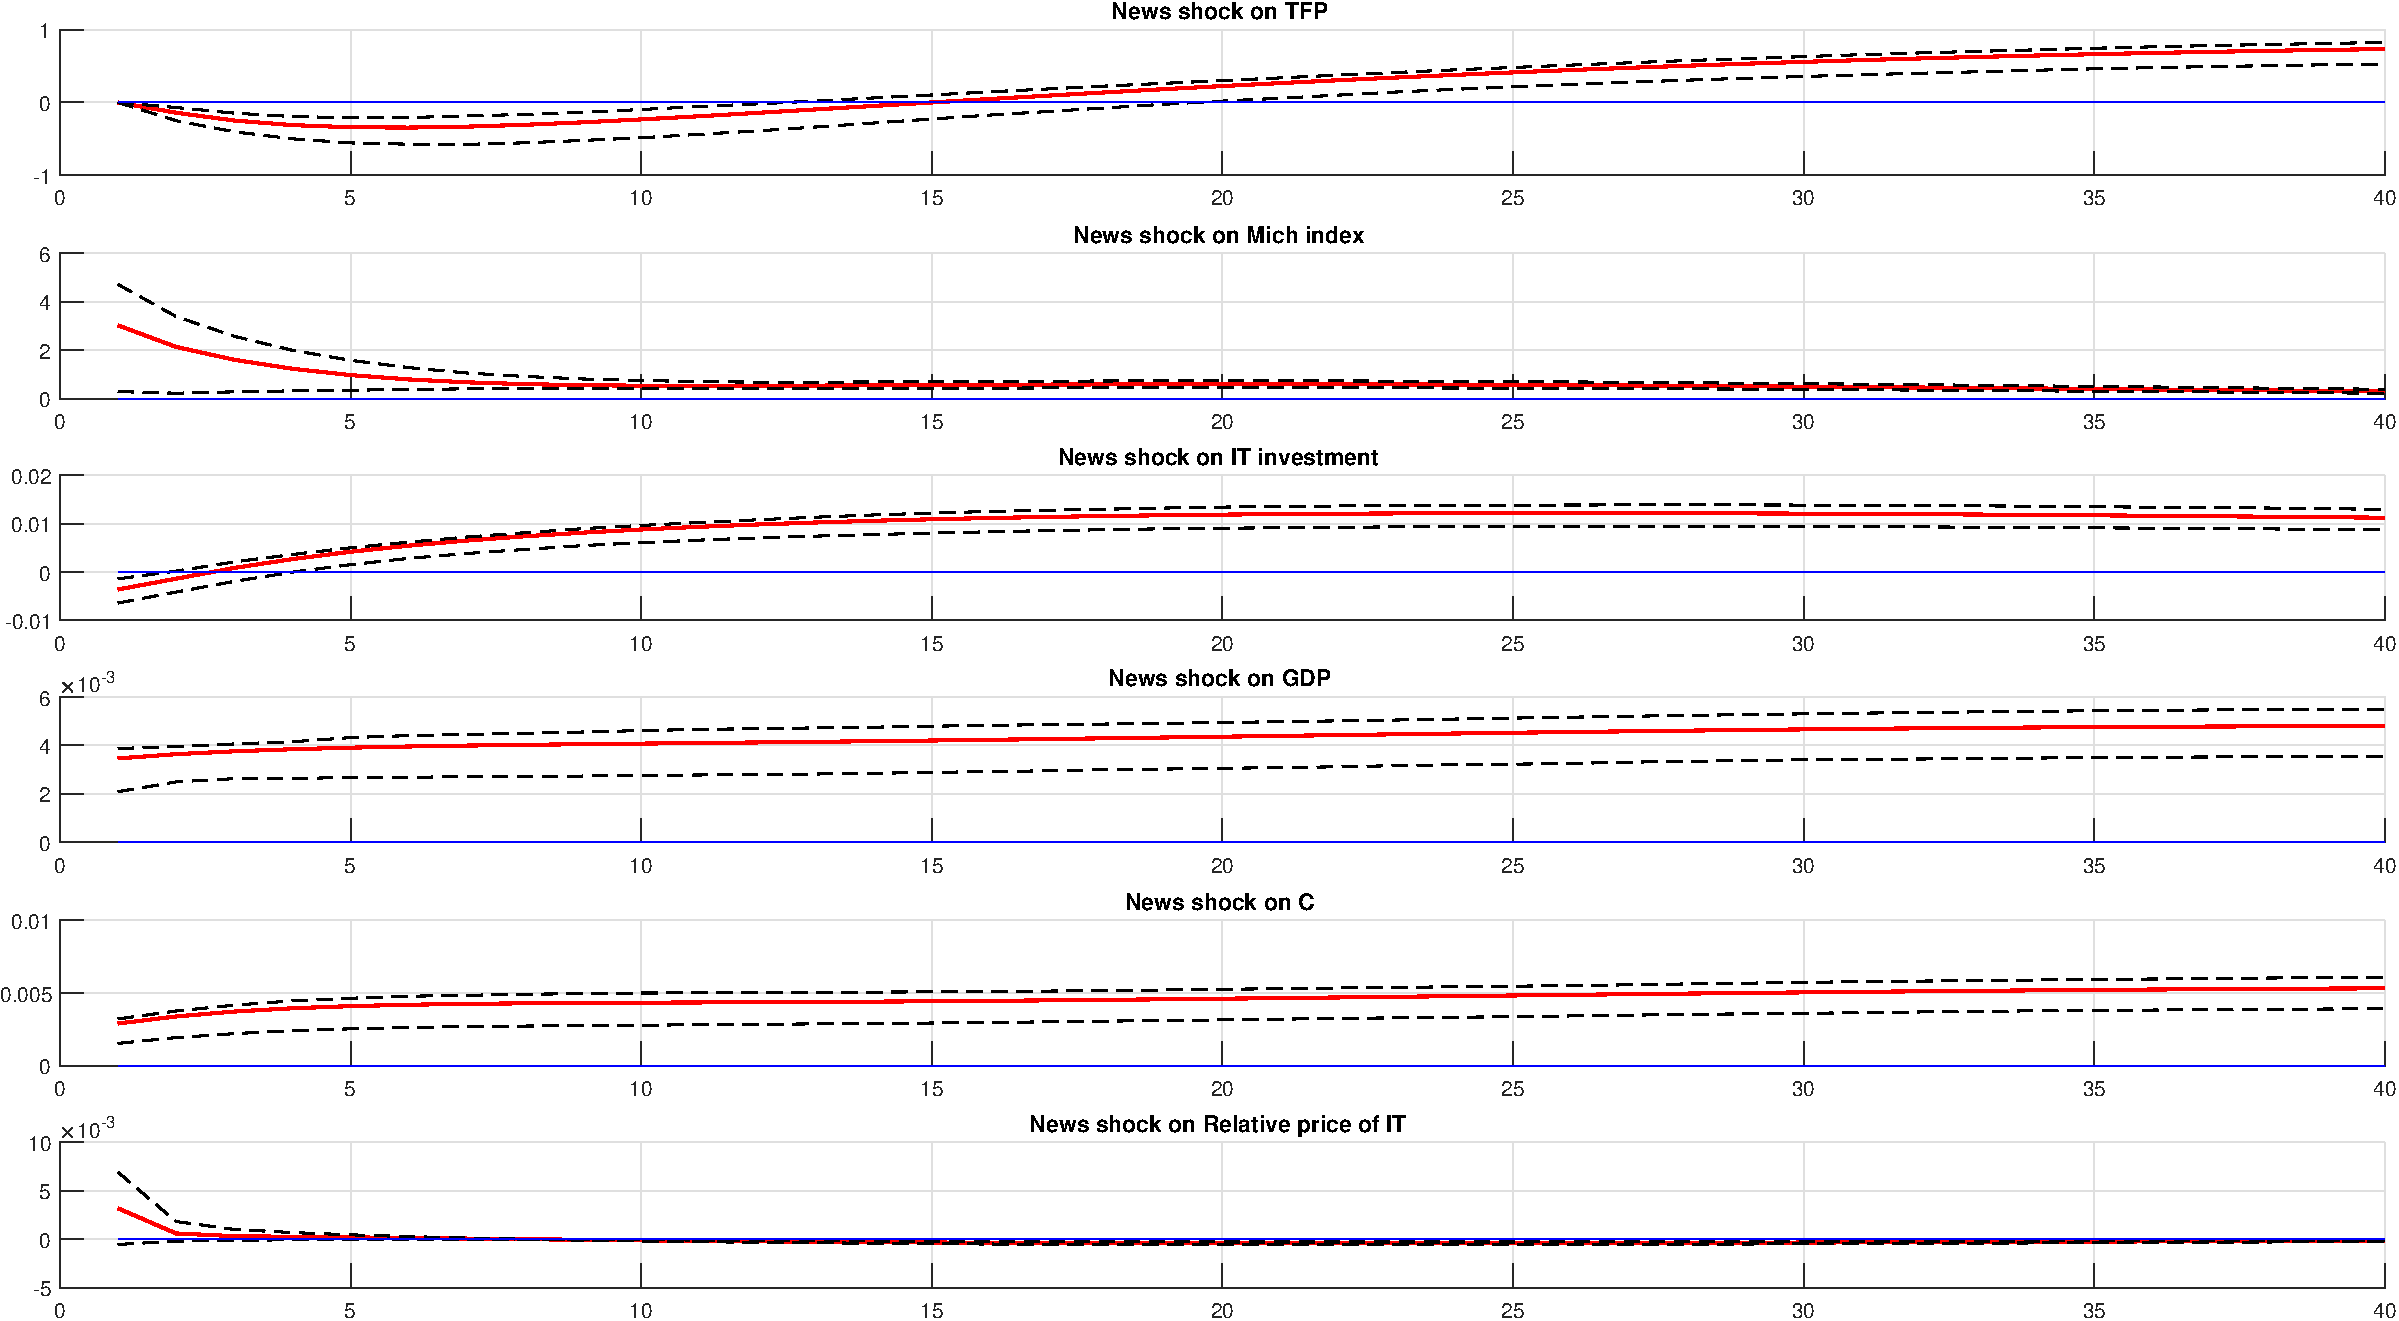
\includegraphics[width=8.5cm]{\ourFigPath Figures/fig_News_shock_Ryan_two_stepsID_20-Nov-2017_12_24_34}} \hspace{.2in%
} 
\subfigure[IT]{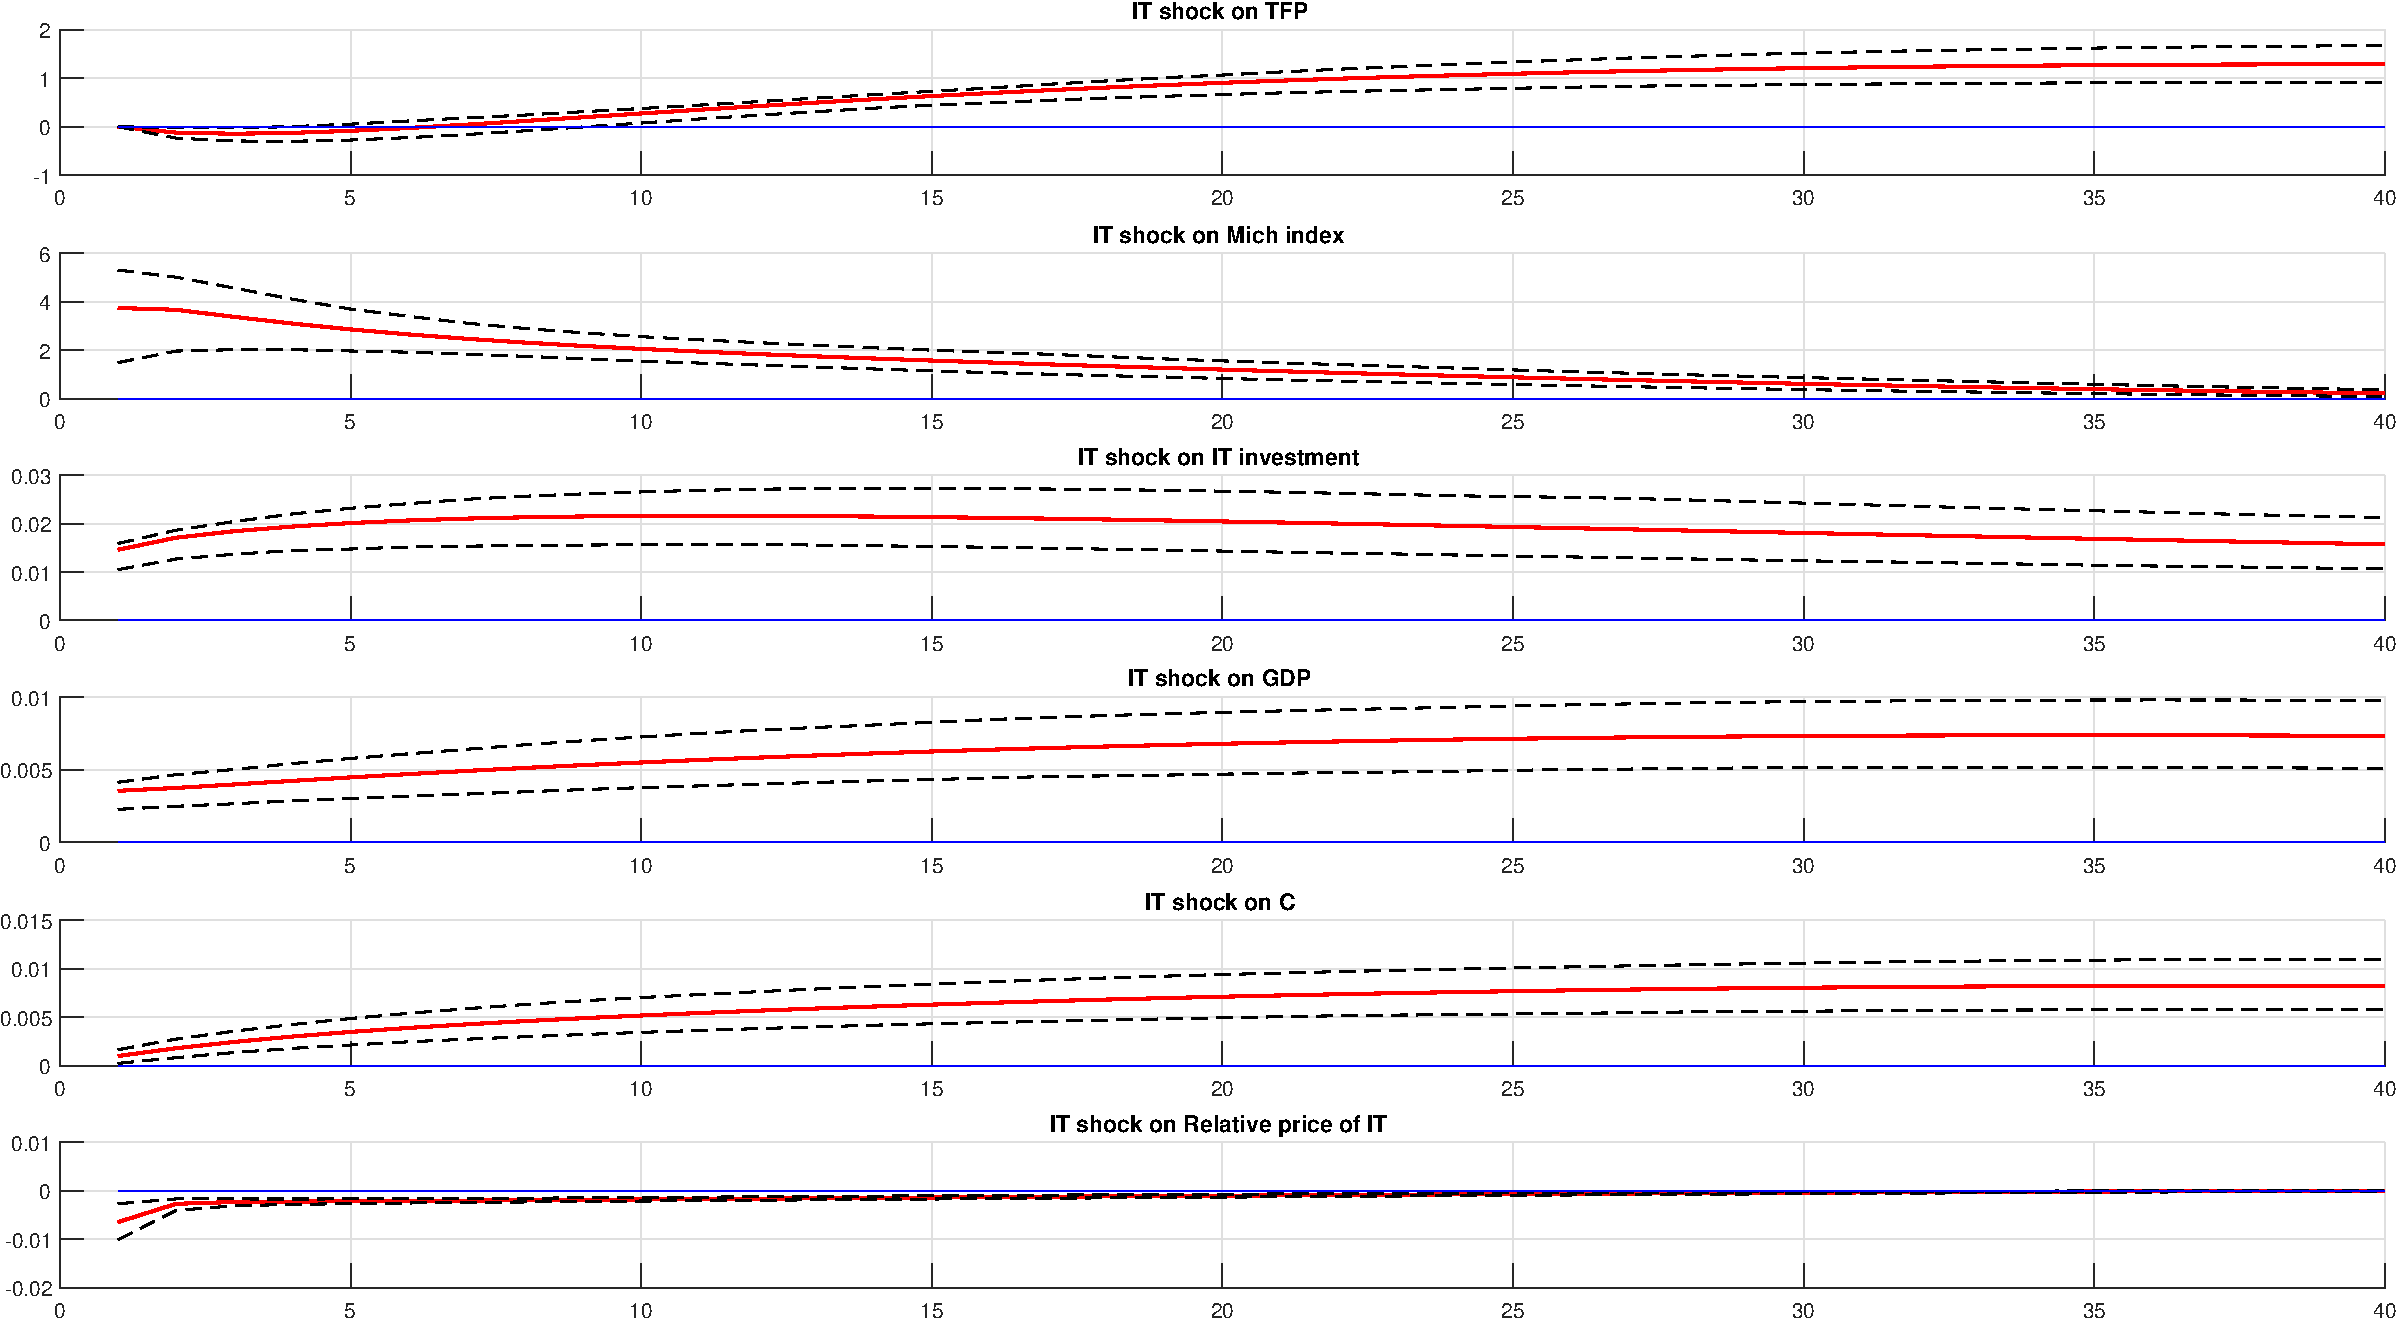
\includegraphics[width=8.5cm]{\ourFigPath Figures/fig_IT_shock_Ryan_two_stepsID_20-Nov-2017_12_24_39}}
\end{figure}
 
%%%%%%%%
% LR hor of 16 
\newpage
\subsection{Relative prices LR horizon 16}
	\noindent Time it took, for 500 bootstrap, Mac: 61 min
	
	\
	
	\noindent  'News'       'IT'        'Total' 
	
         \noindent  '0.10054'    '0.60847'    '0.70901'
         
         \
         
         \begin{small}
	\begin{tabular}{lccc}
	\hline
		& News & IT & Total \\
		\hline
		Share of TFP FEV explained & 0.1 & 0.6 & 0.7 \\
		\hline
	\end{tabular}
\end{small}

         
         \

\begin{figure}[h!]
\centering
\subfigure[News]{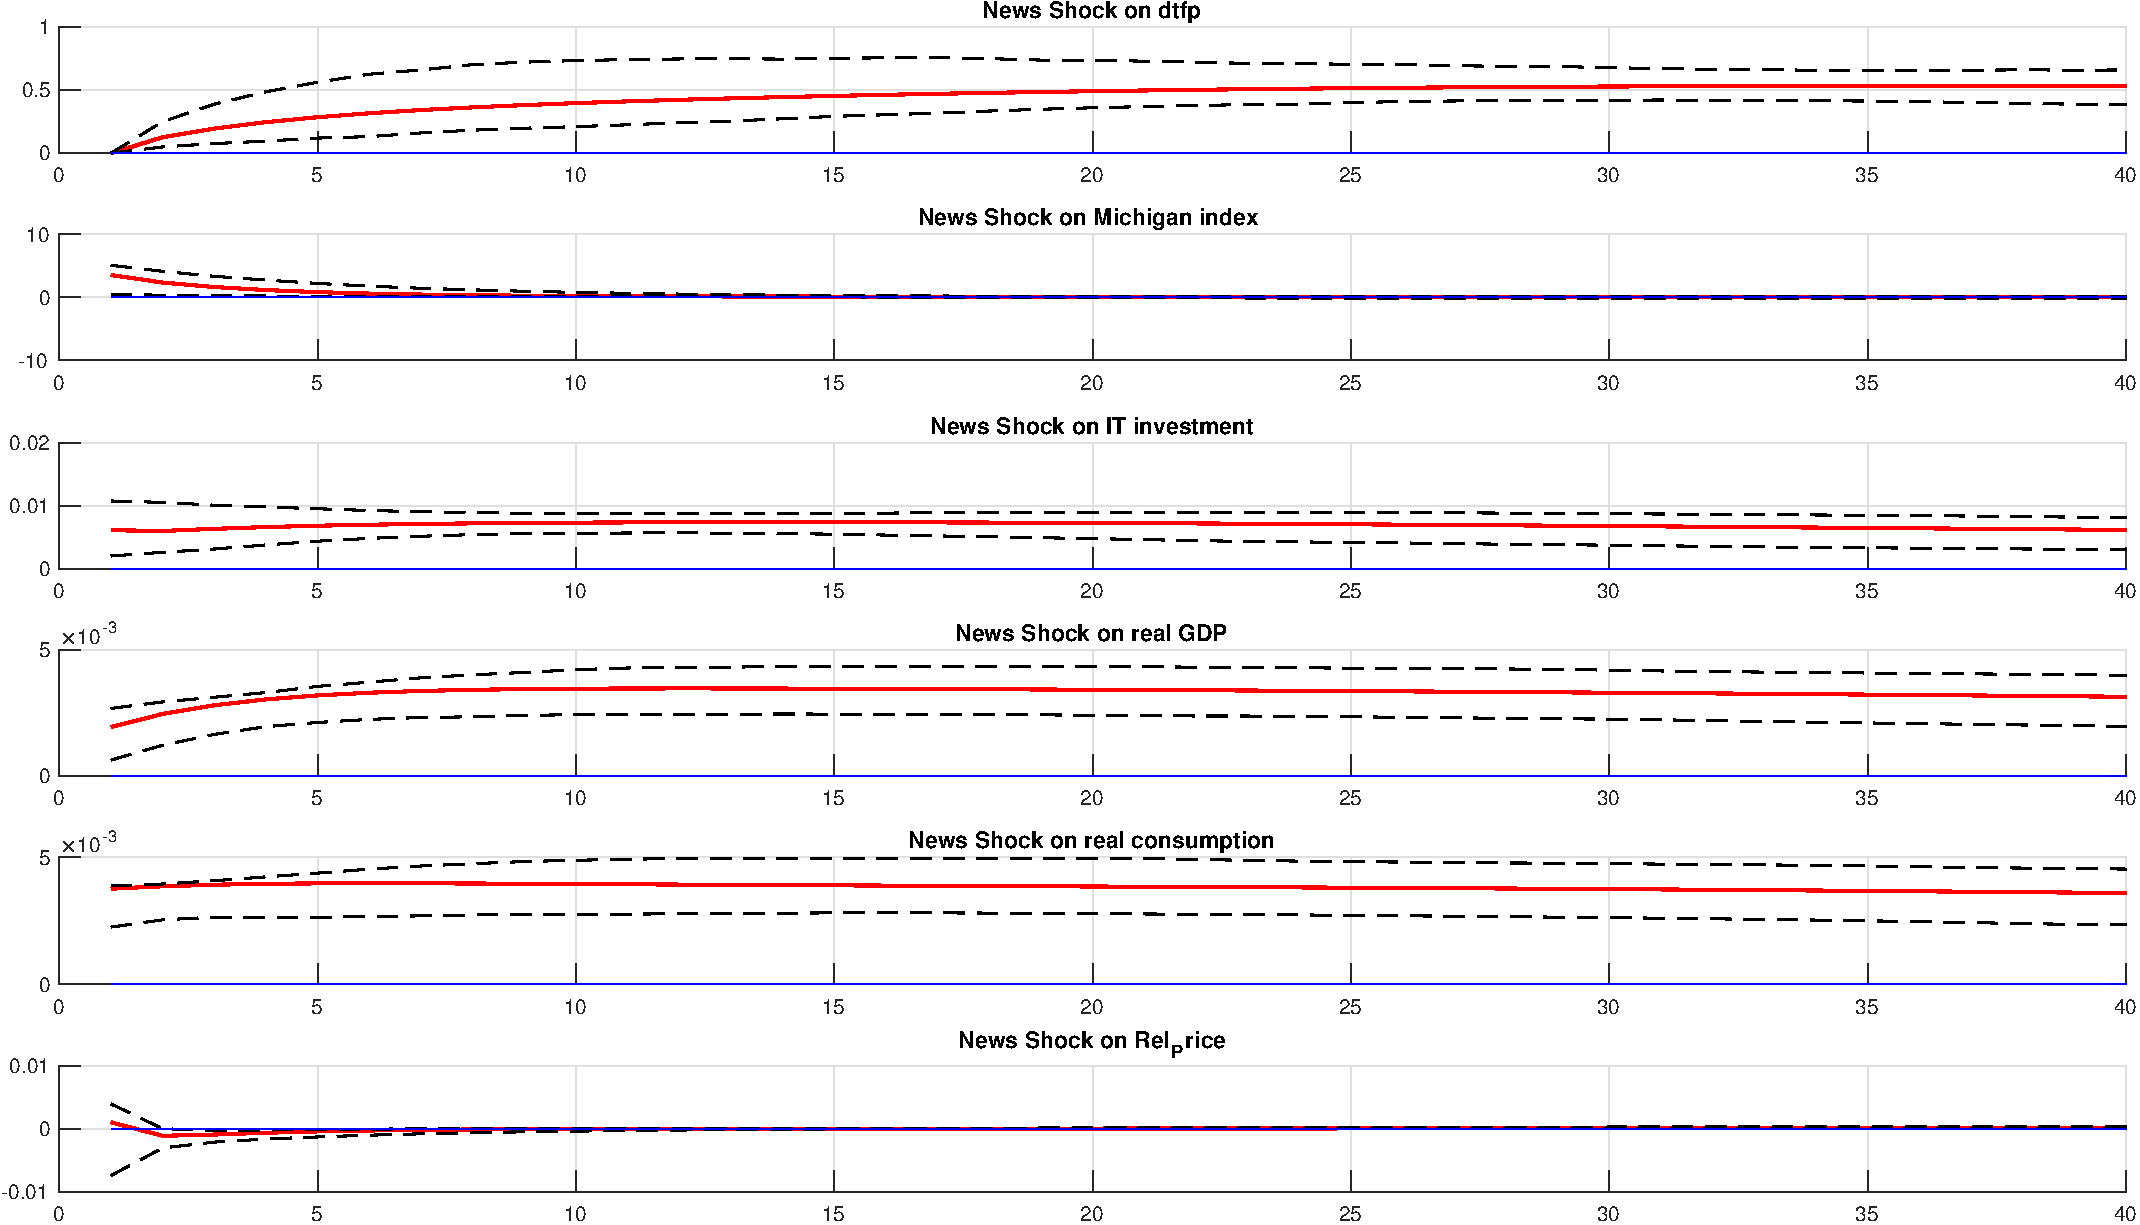
\includegraphics[width=8.5cm]{\ourFigPath Figures/fig_News_Shock_Ryan_two_stepsID_24-Nov-2017_18_56_19}} \hspace{.2in%
} 
\subfigure[IT]{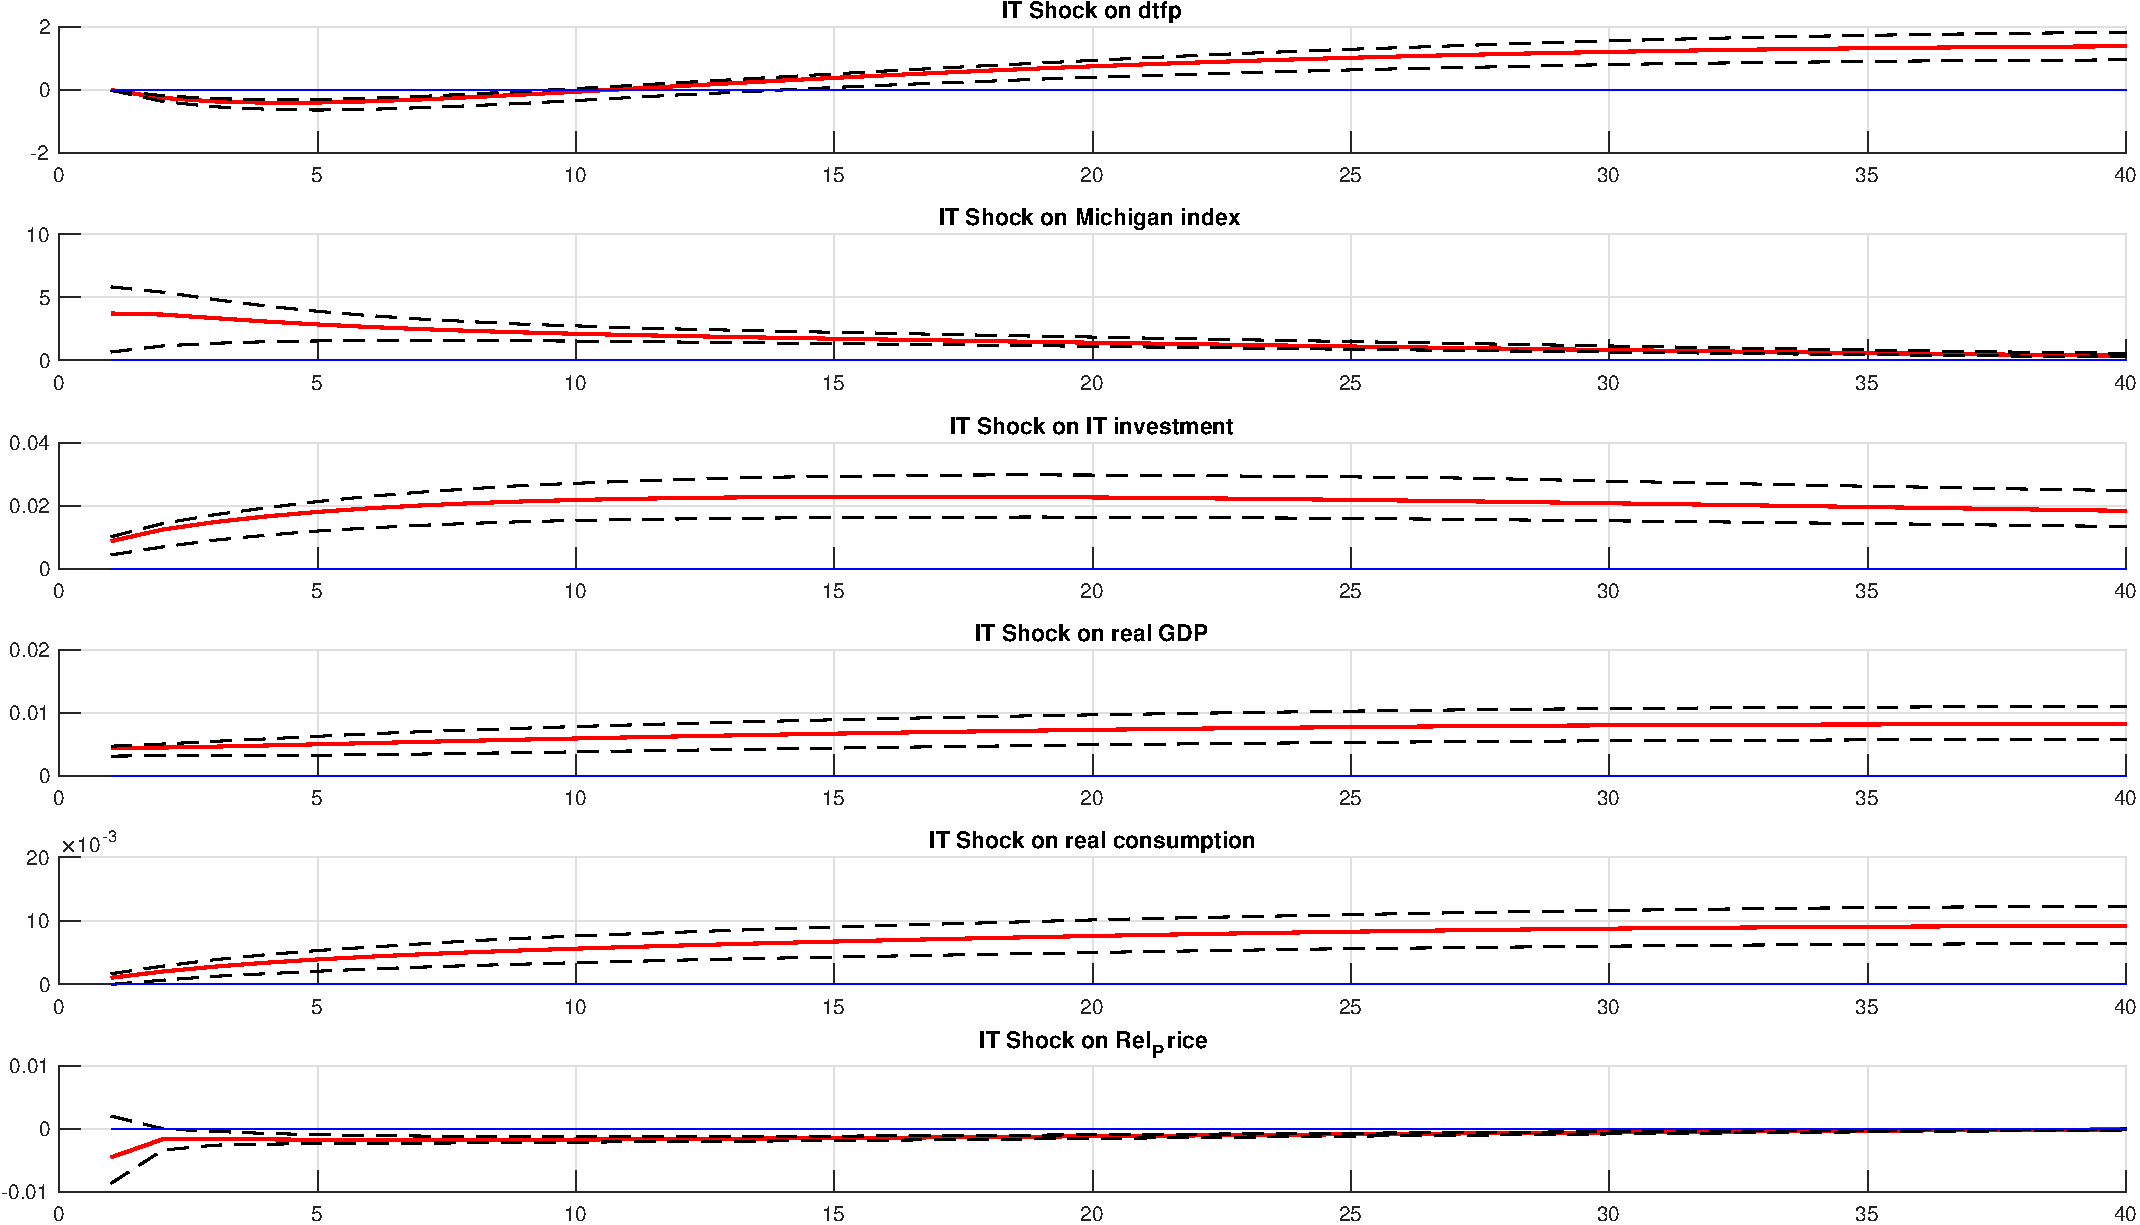
\includegraphics[width=8.5cm]{\ourFigPath Figures/fig_IT_Shock_Ryan_two_stepsID_24-Nov-2017_18_56_23}}
\end{figure}


%%%%%%%%
% LR hor of 80 - 
\newpage
\subsection{Relative prices LR horizon 80}
	\noindent Time it took, for 500 bootstrap, Mac: 81 min
	
	\
	
	\noindent  'News'       'IT'        'Total' 
	
         \noindent  '0.044546'    '0.69612'    '0.74067'
         
         \
         
         \begin{small}
	\begin{tabular}{lccc}
	\hline
		& News & IT & Total \\
		\hline
		Share of TFP FEV explained & 0.0 & 0.7 & 0.7 \\
		\hline
	\end{tabular}
\end{small}

         
         \

\begin{figure}[h!]
\centering
\subfigure[News]{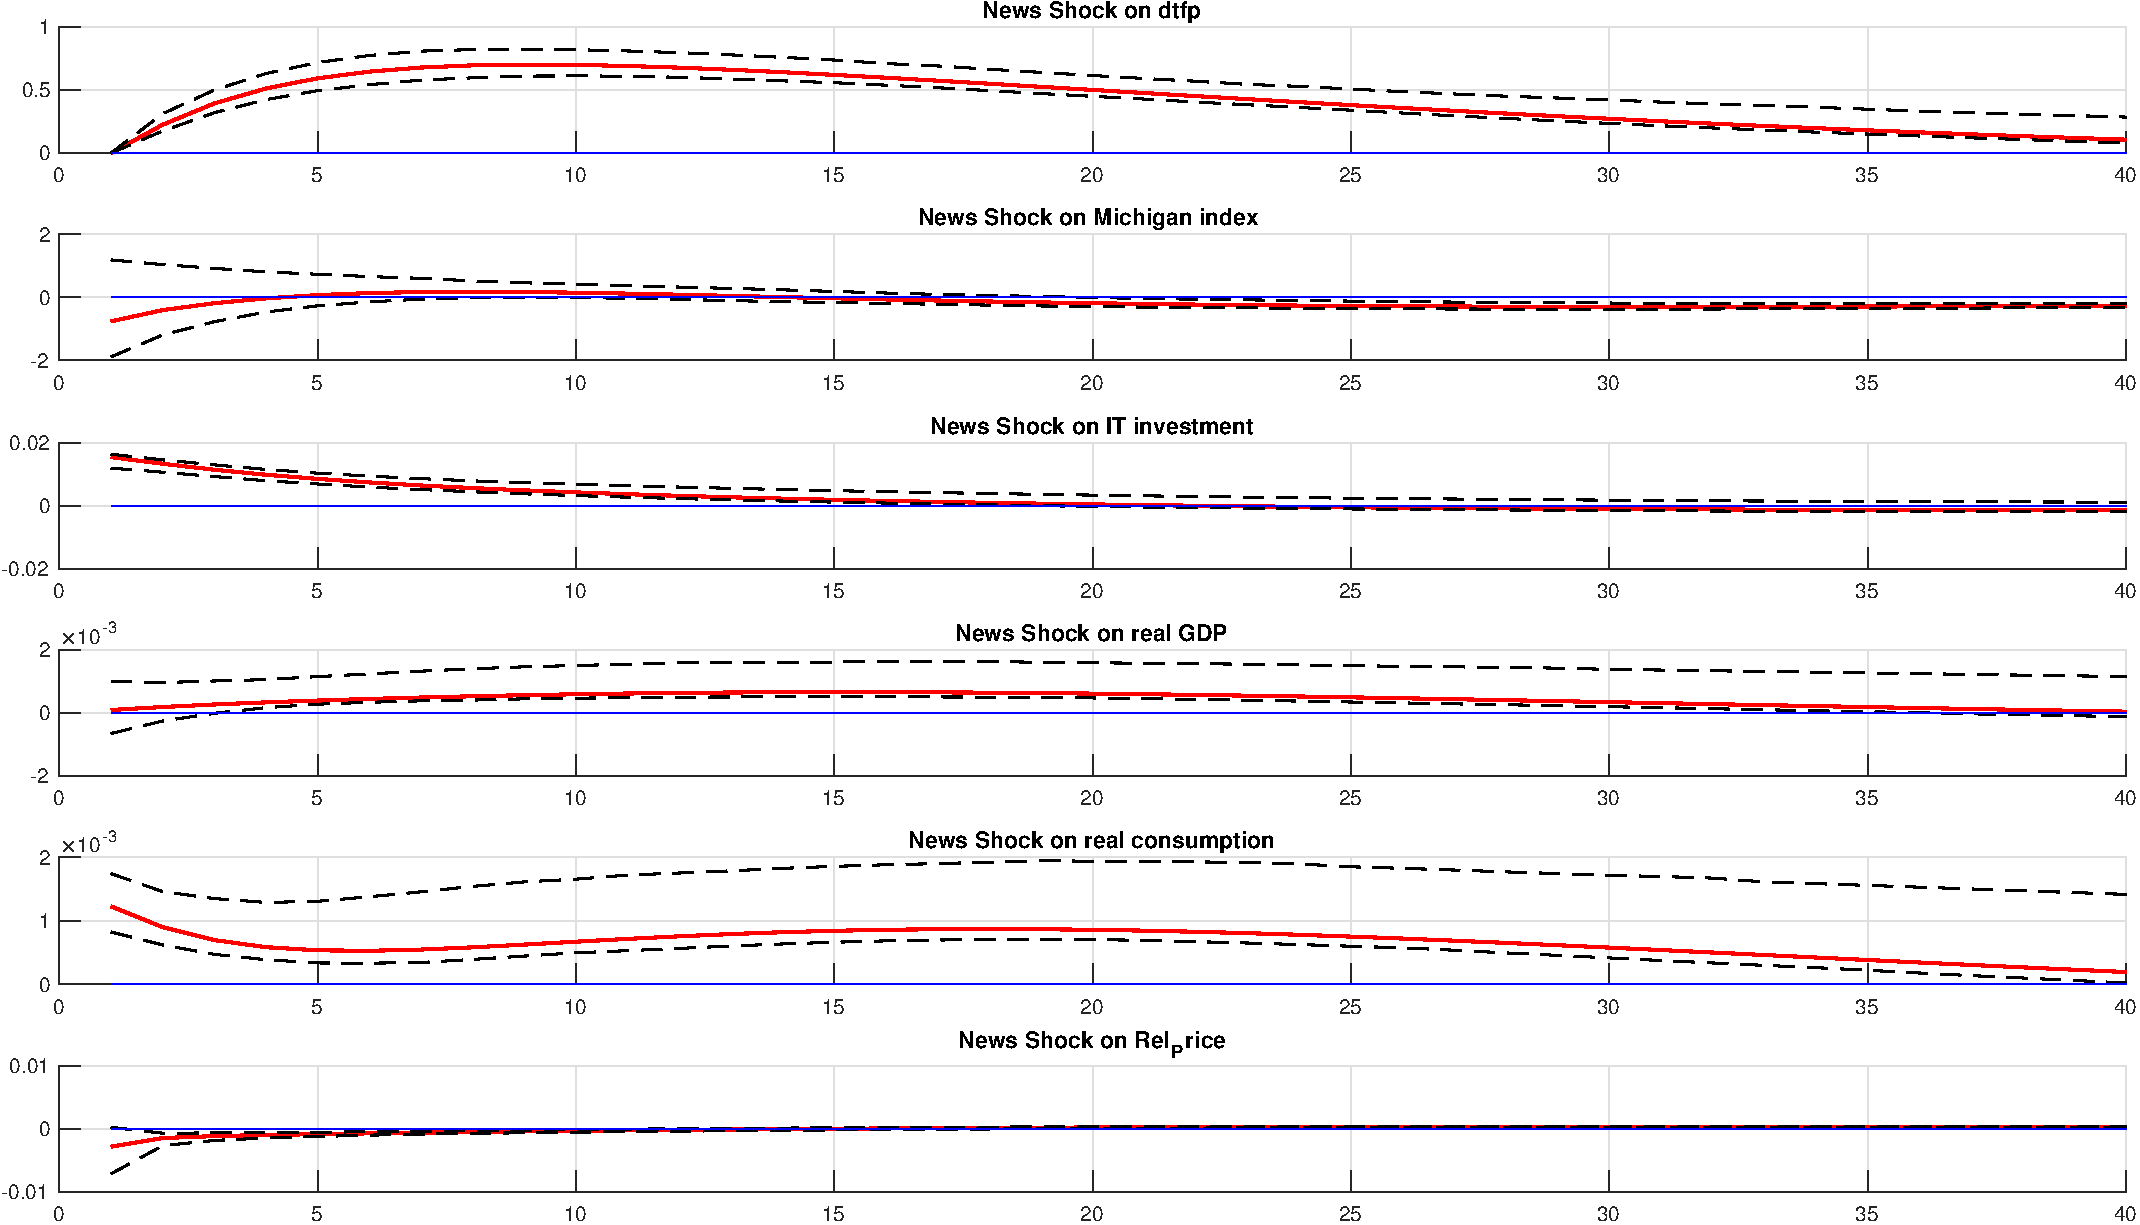
\includegraphics[width=8.5cm]{\ourFigPath Figures/fig_News_Shock_Ryan_two_stepsID_24-Nov-2017_21_59_10}} \hspace{.2in%
} 
\subfigure[IT]{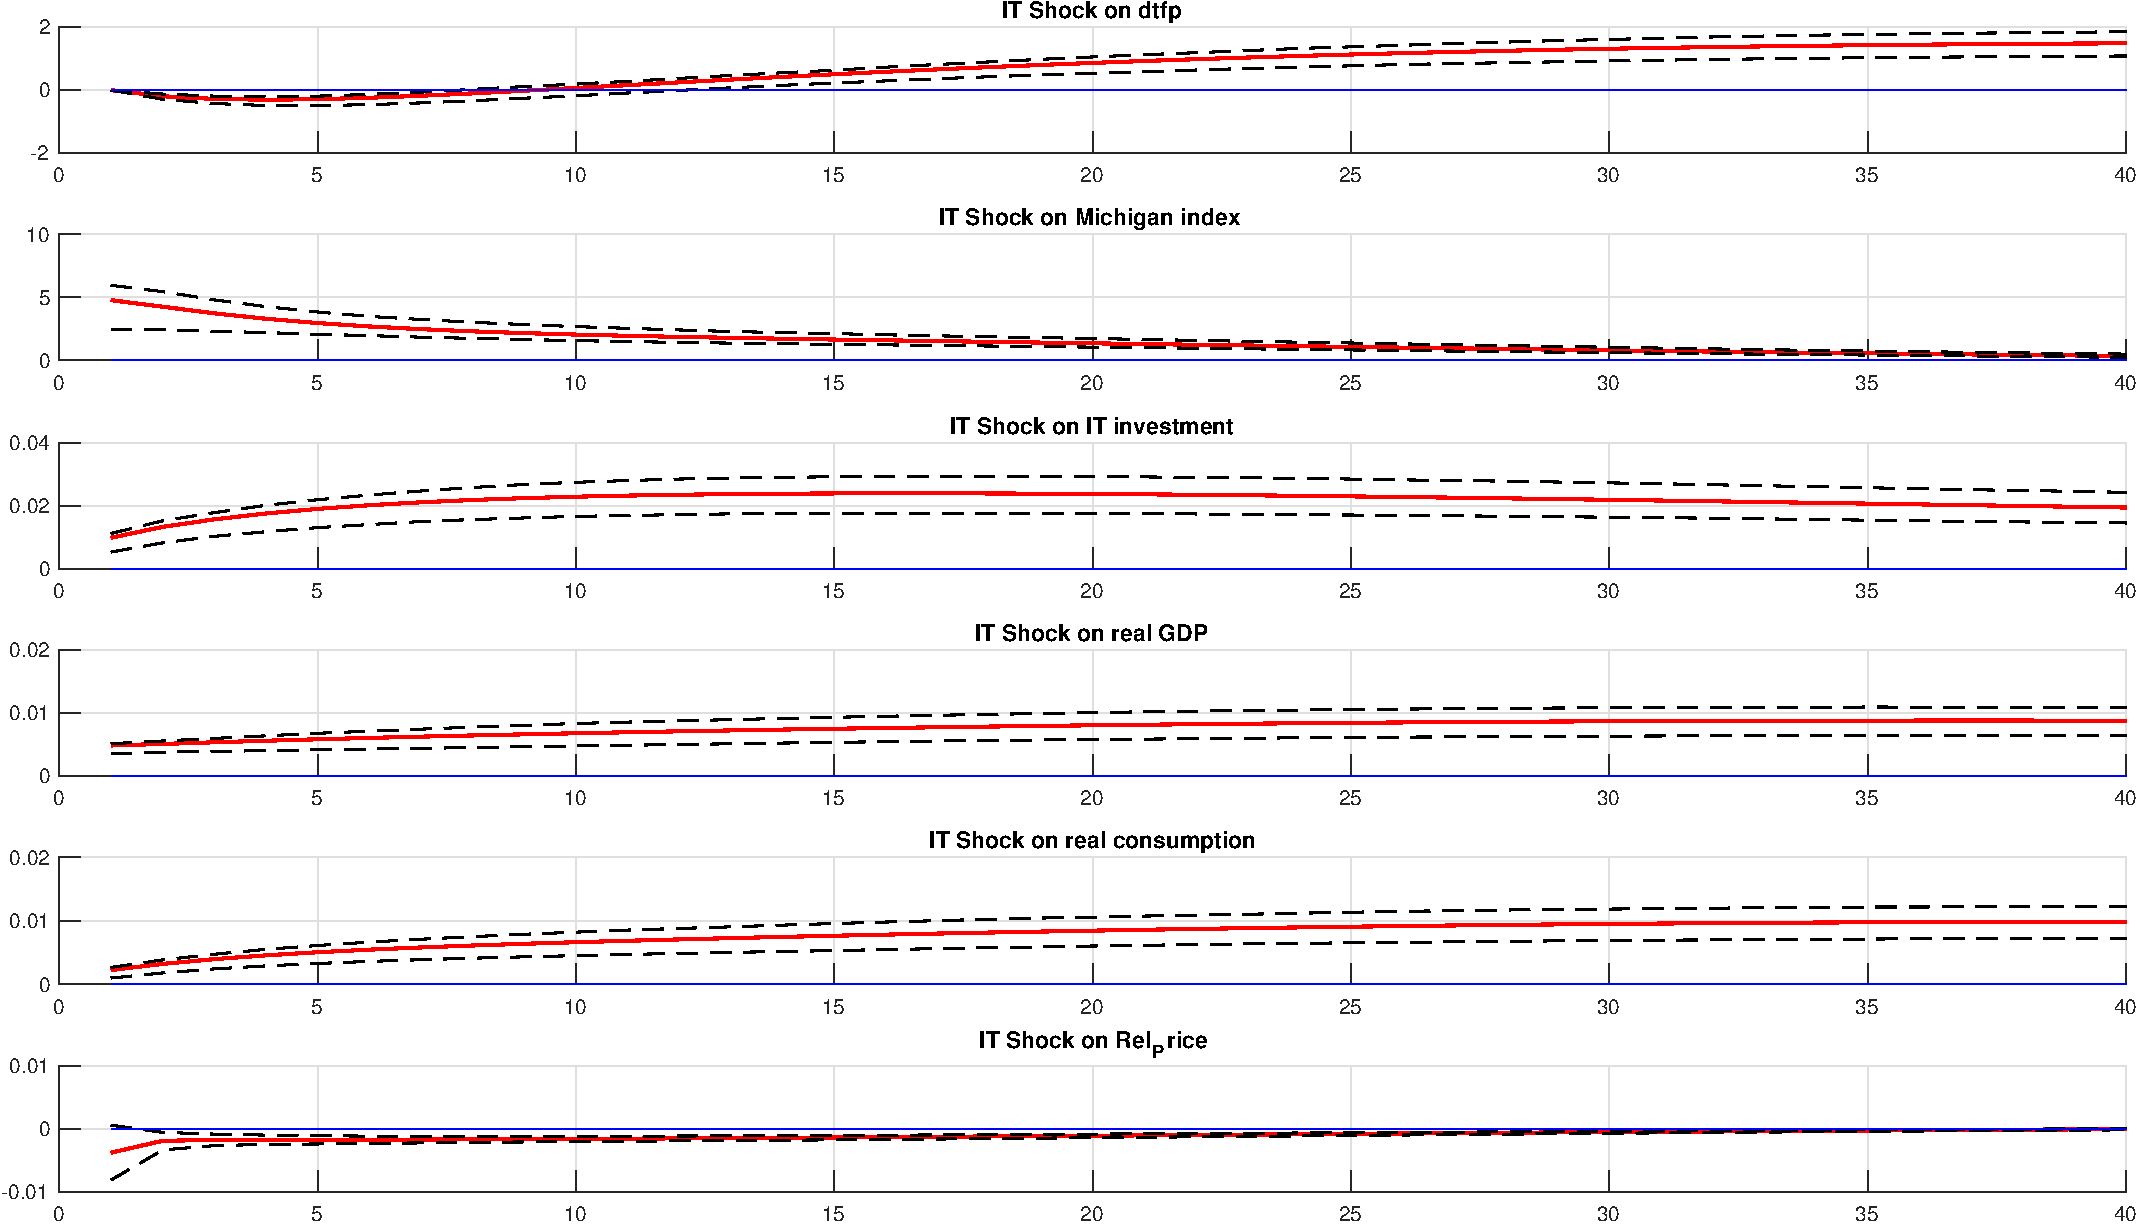
\includegraphics[width=8.5cm]{\ourFigPath Figures/fig_IT_Shock_Ryan_two_stepsID_24-Nov-2017_21_59_14}}
\end{figure}
 
%%%%%%%%
%one lag (back to LR hor = 8), adding real stock prices 500, removing GDP, with relative price
\newpage
	\subsection{Relative prices LR horizon 8, adding SP 500}
	\noindent one lag, LR hor = 8, adding real stock prices 500, removing GDP, with relative price
	
	
	\begin{small}
	\begin{tabular}{lccc}
	\hline
		& News & IT & Total \\
		\hline
		Share of TFP FEV explained & 0.45829 & 0.40823 & 0.86651 \\
		\hline
	\end{tabular}
\end{small}

	
	\begin{figure}[h!]
\centering
\subfigure[News]{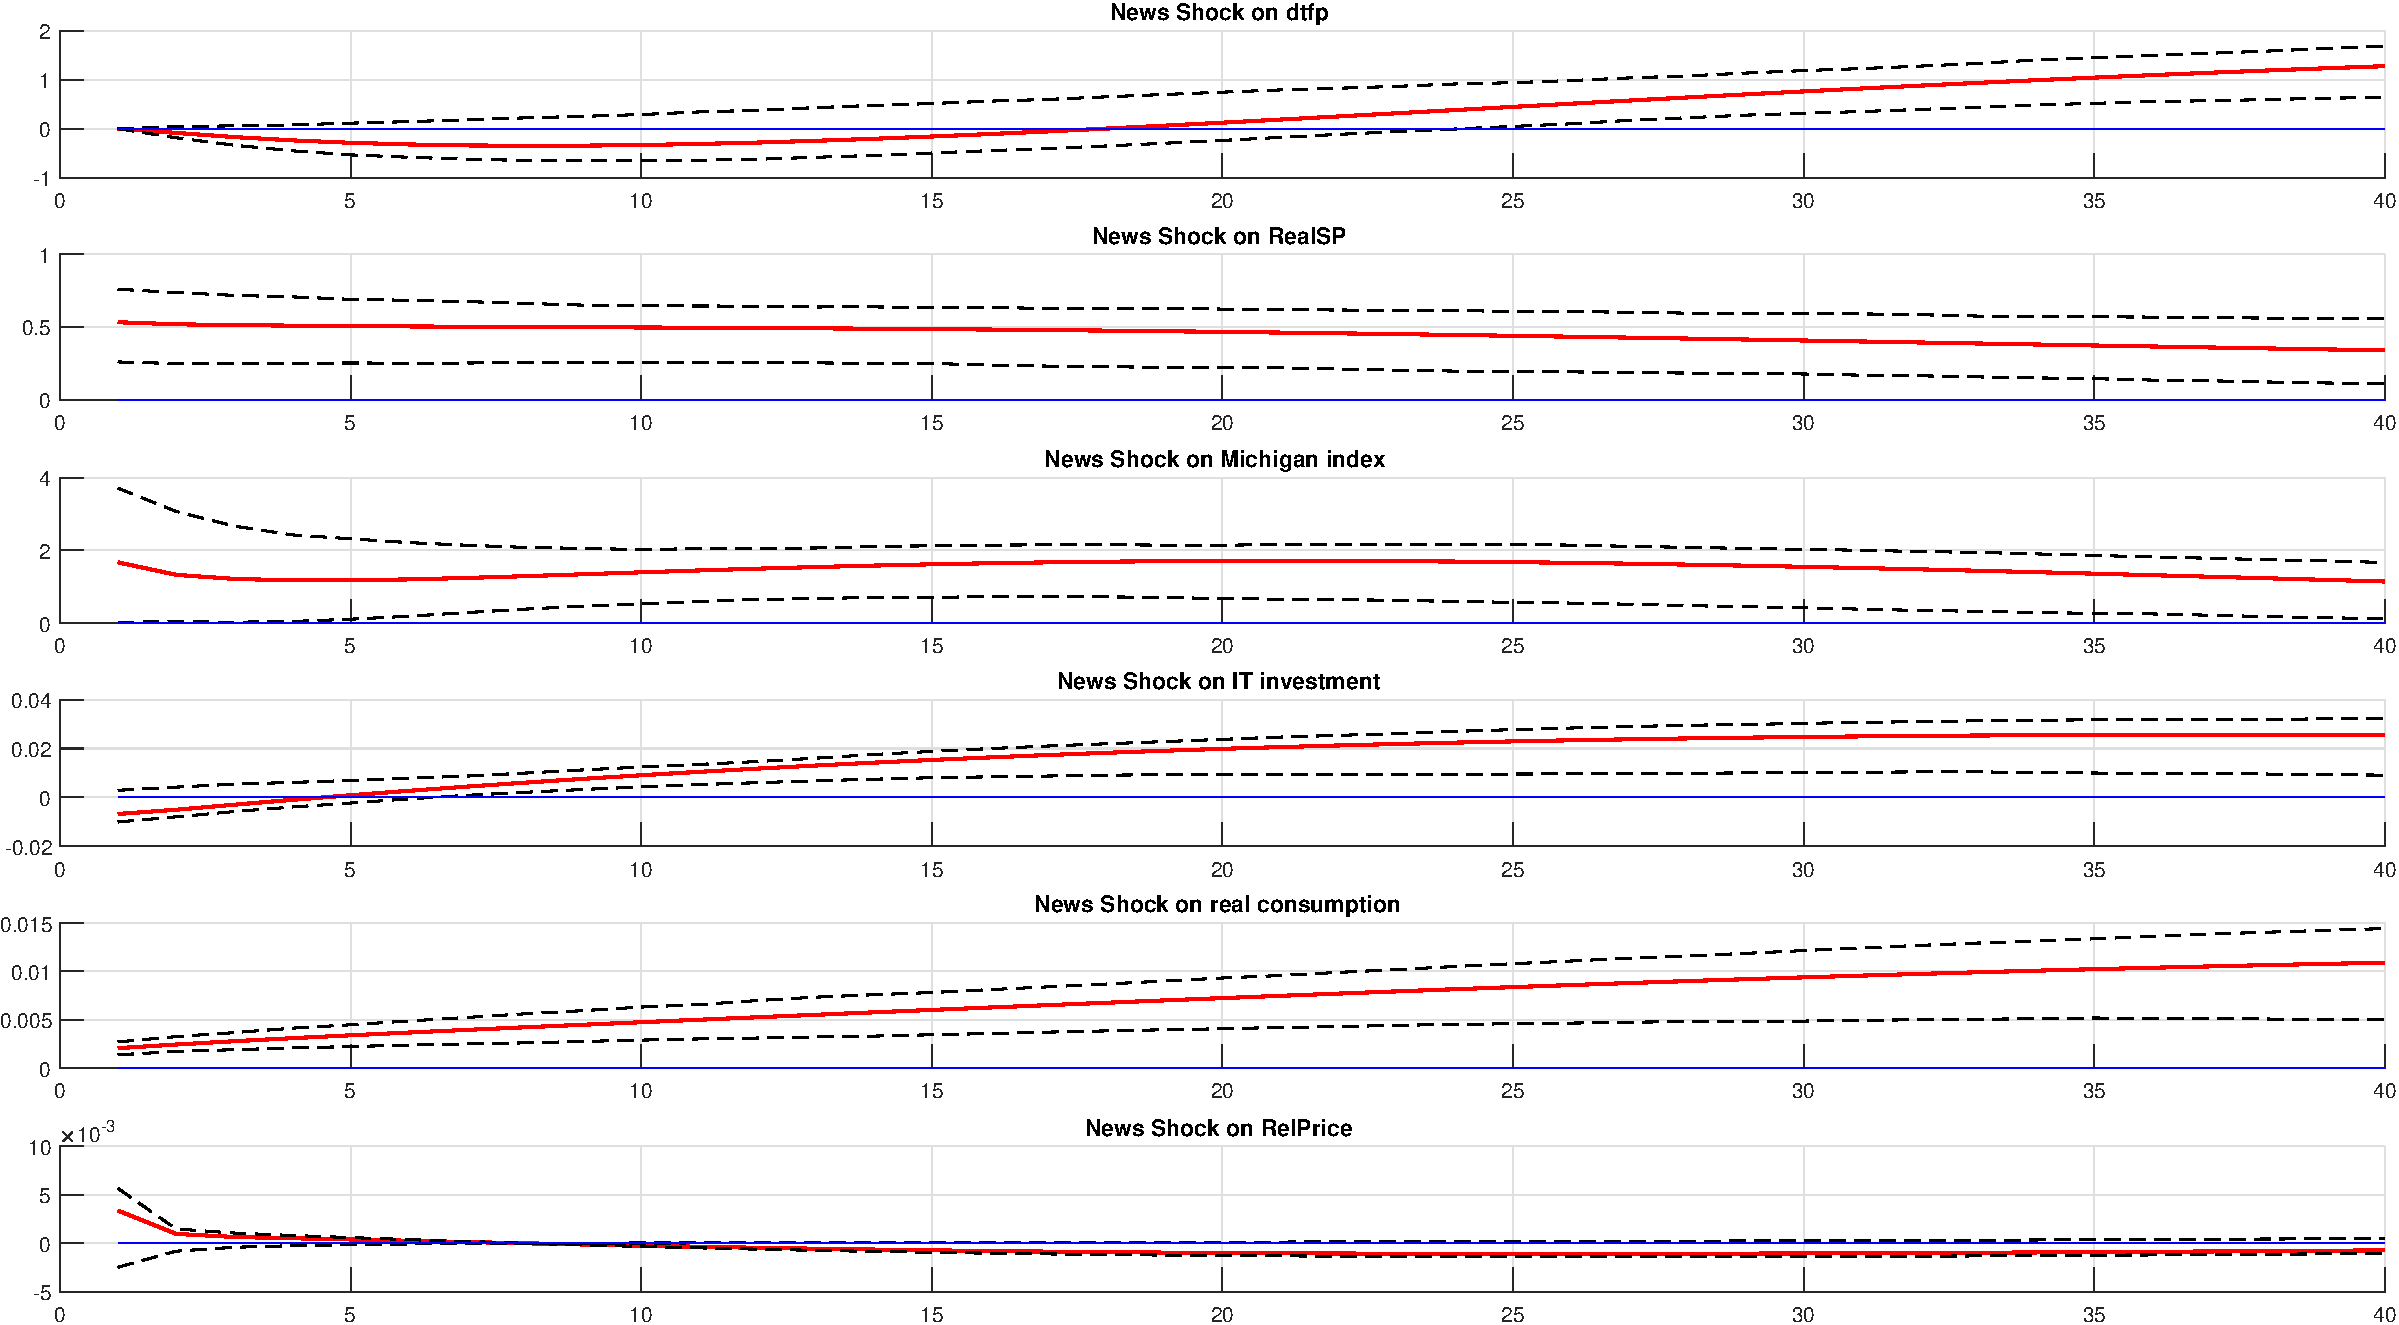
\includegraphics[width=8.5cm]{\ourFigPath Figures/fig_News_Shock_Ryan_two_stepsID_25-Nov-2017_11_30_49}} \hspace{.2in%
} 
\subfigure[IT]{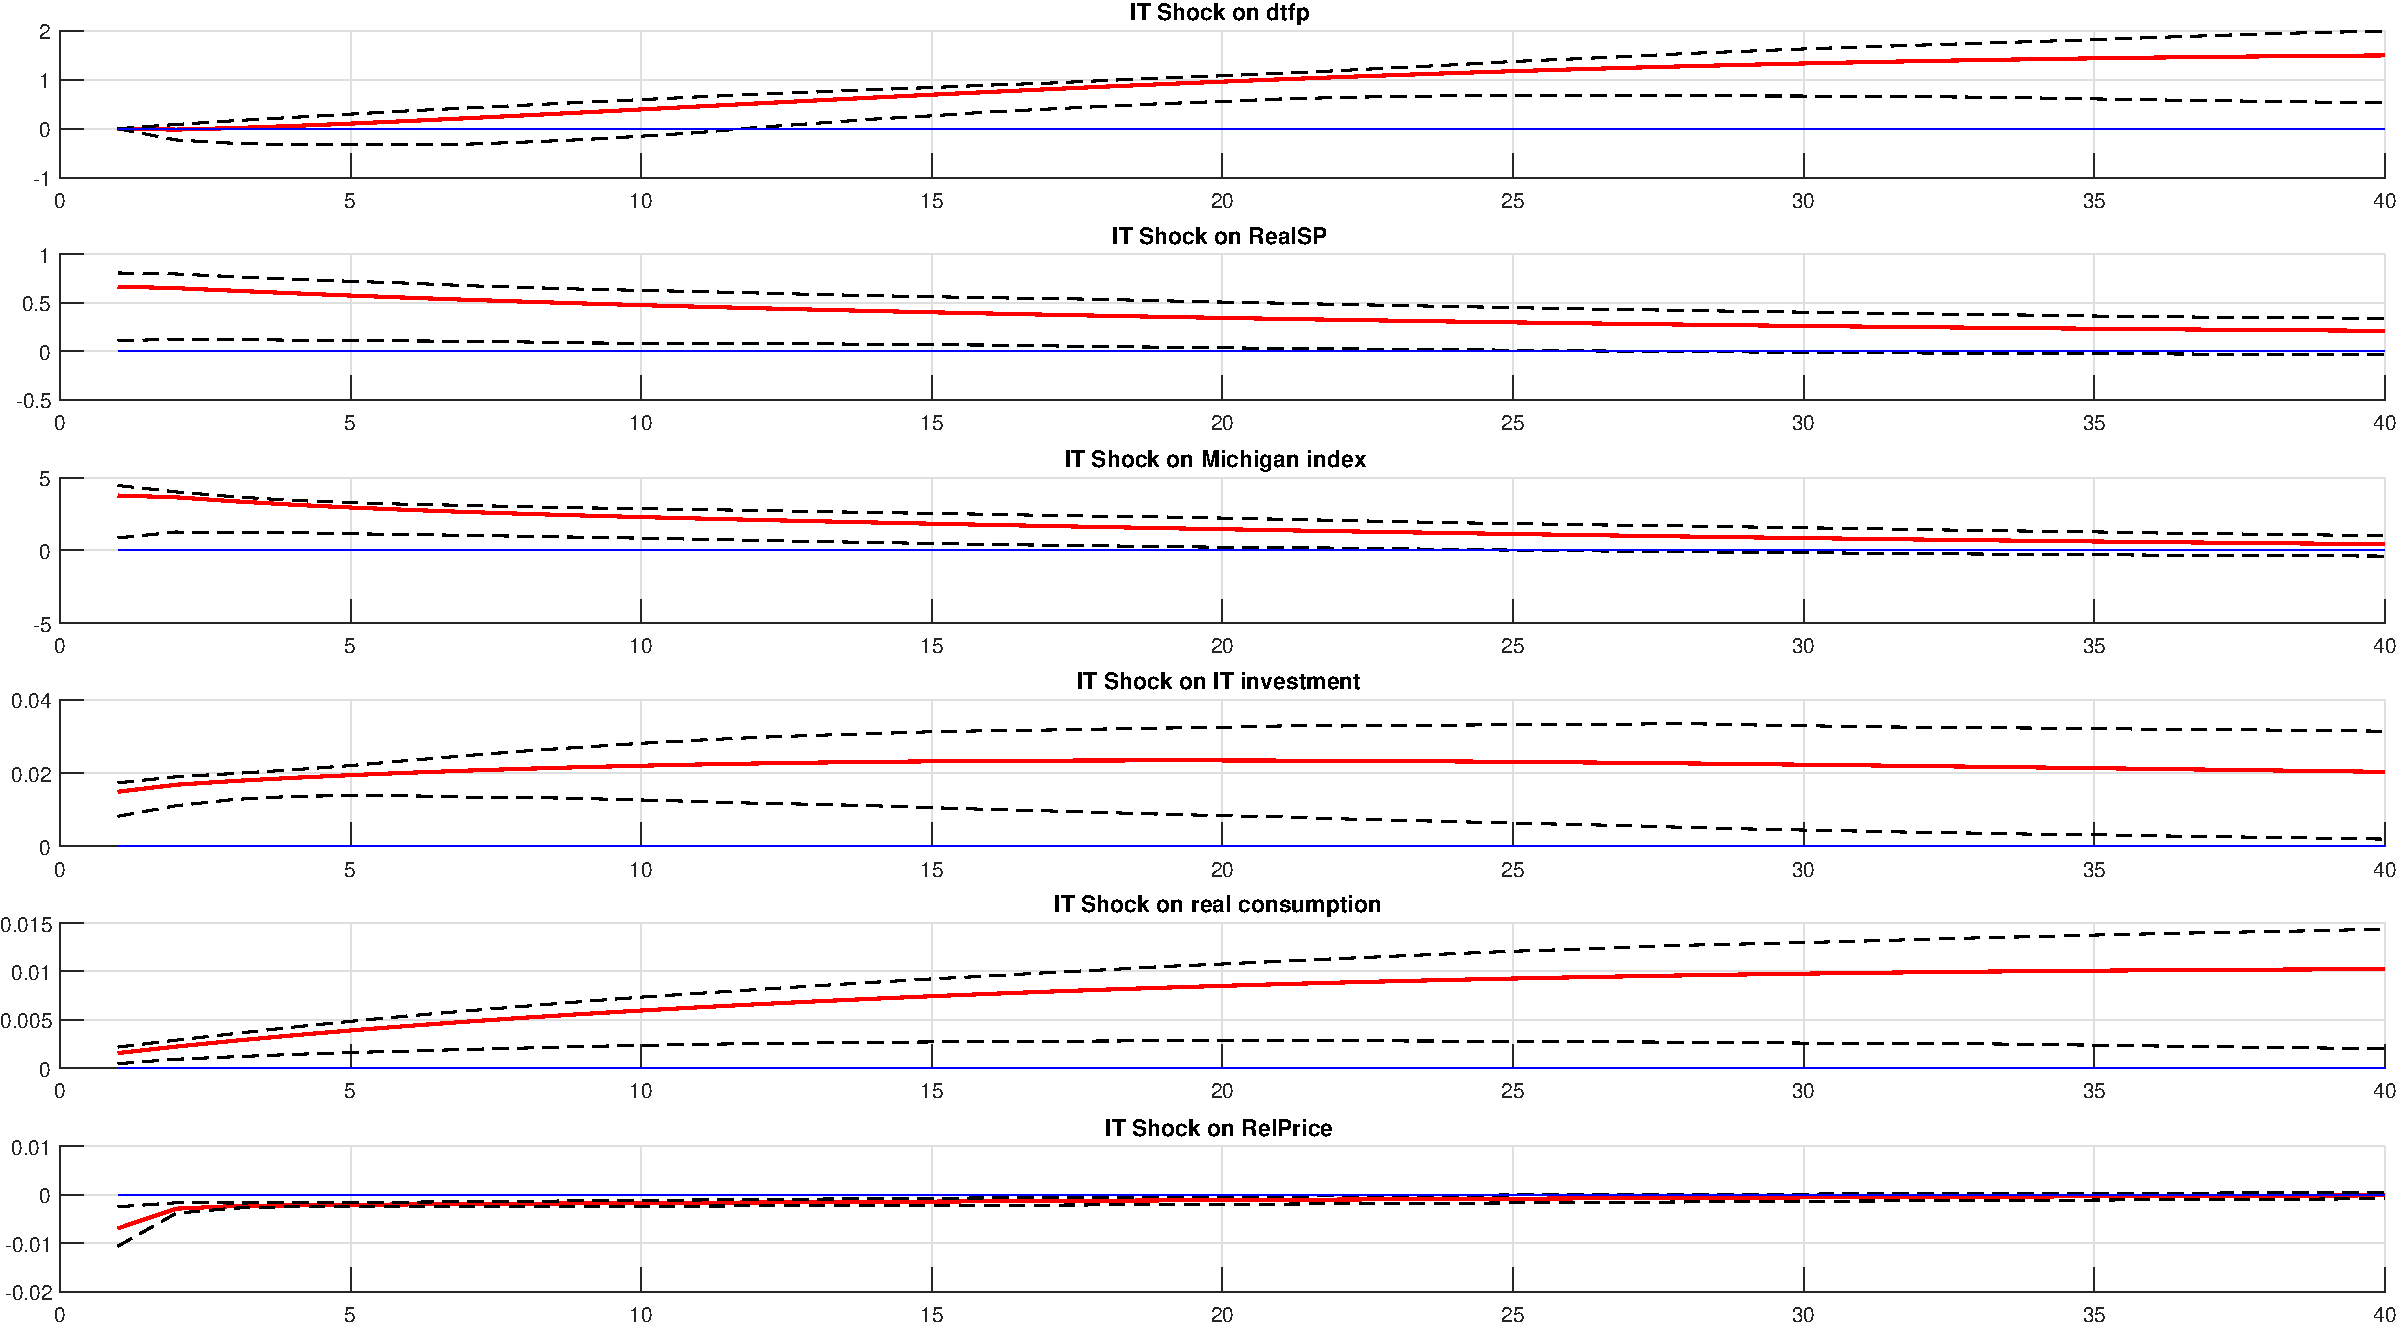
\includegraphics[width=8.5cm]{\ourFigPath Figures/fig_IT_Shock_Ryan_two_stepsID_25-Nov-2017_11_30_52}}
\end{figure}

%%%%%%%%
% adding real SP500, but with GDP
\newpage
	\subsection{Relative prices LR horizon 8, adding SP 500 and leaving in GDP}
	\noindent one lag, LR hor = 8, adding real stock prices 500, leaving in GDP, with relative price; only 30 bootstrap
	
	
	\begin{small}
	\begin{tabular}{lccc}
	\hline
		& News & IT & Total \\
		\hline
		Share of TFP FEV explained & 0.3 & 0.6 & 0.8 \\
		\hline
	\end{tabular}
\end{small}

	
	\begin{figure}[h!]
\centering
\subfigure[News]{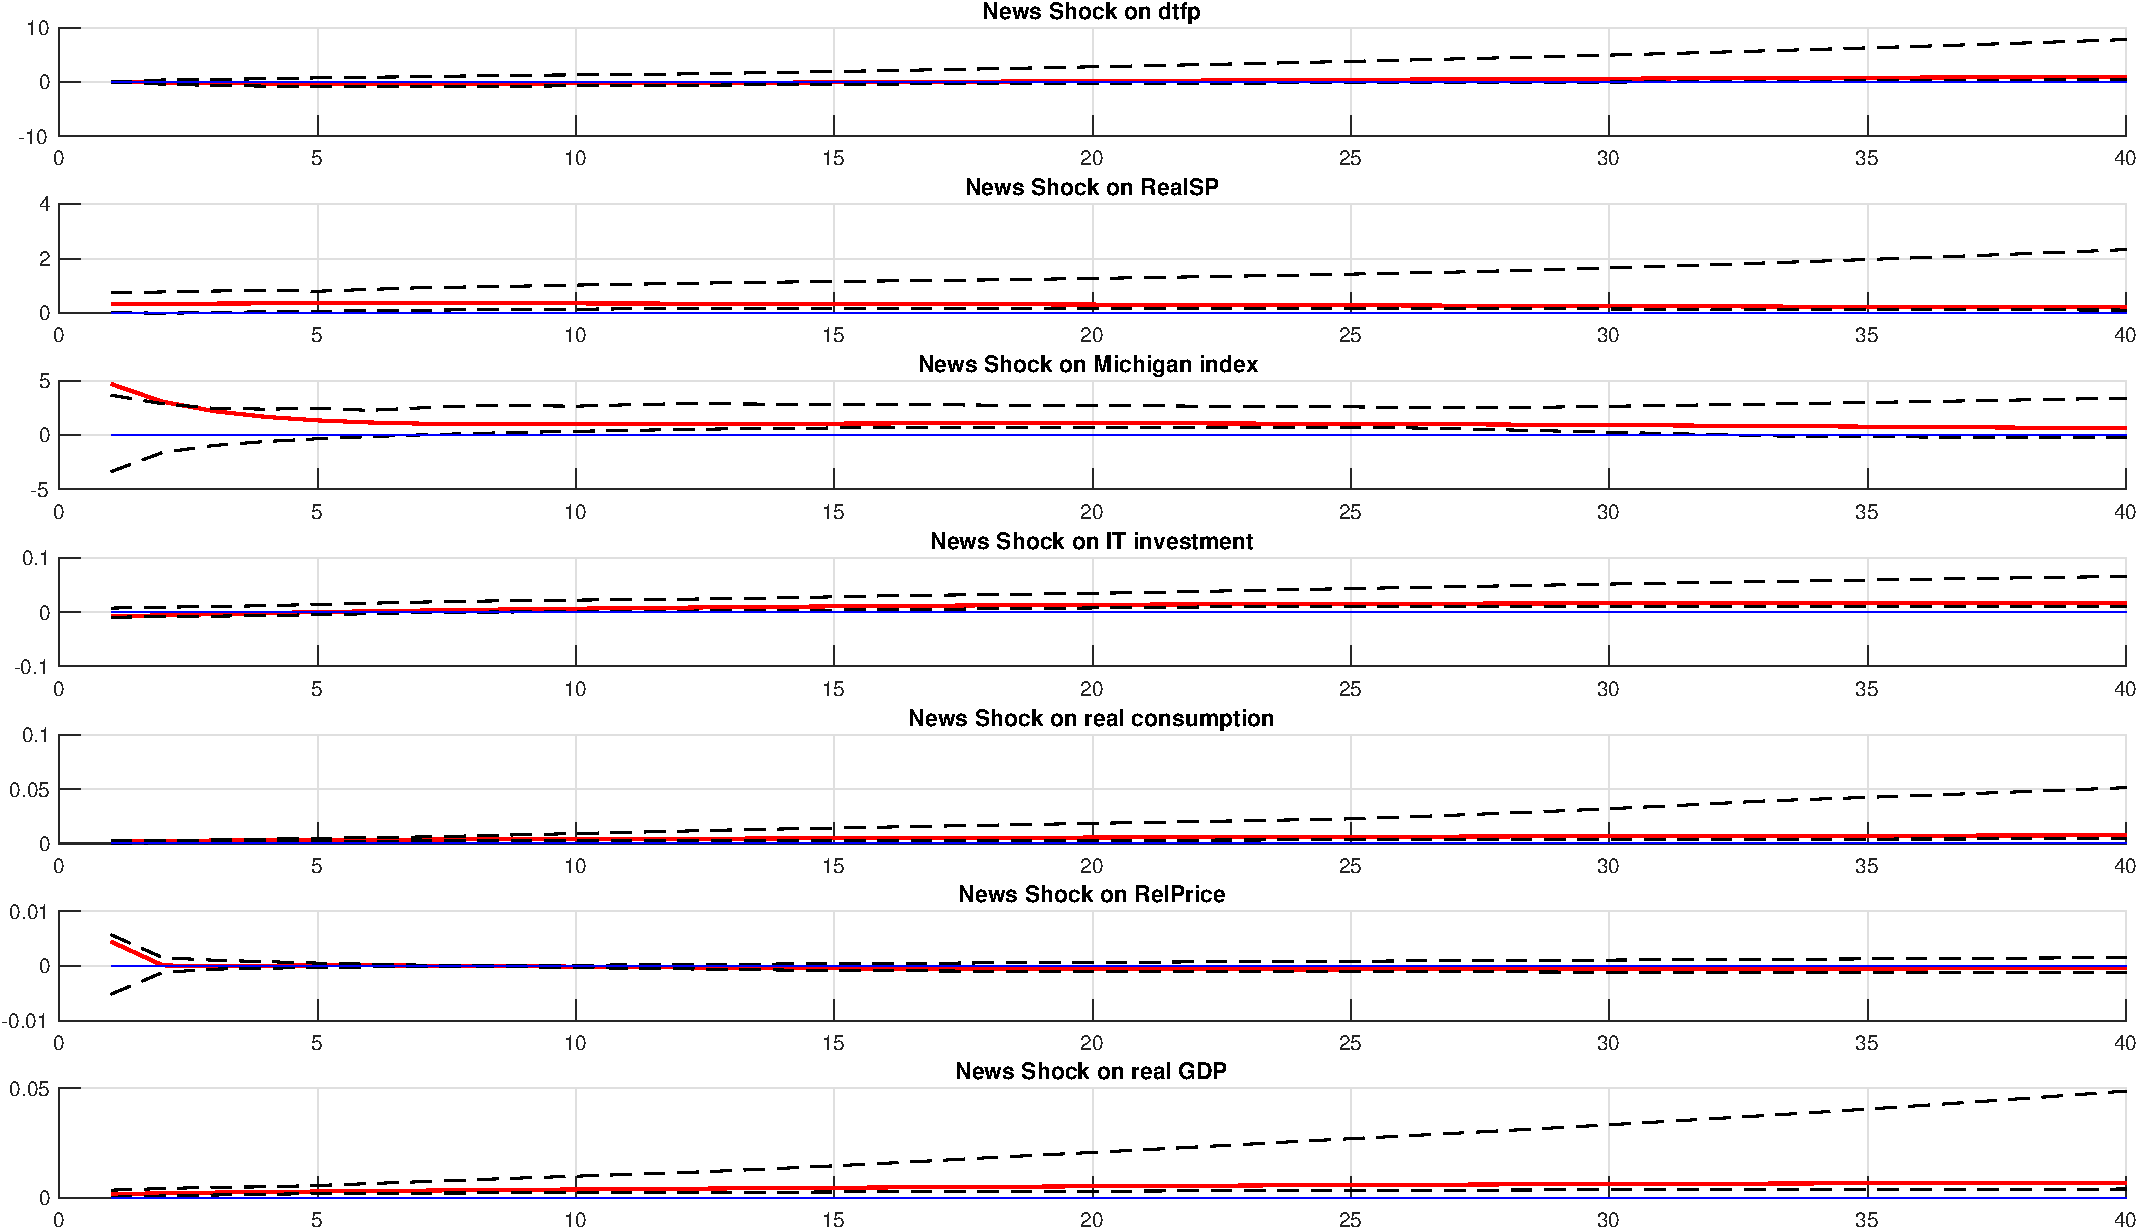
\includegraphics[width=8.5cm]{\ourFigPath Figures/fig_News_Shock_Ryan_two_stepsID_26-Nov-2017_09_36_04}} \hspace{.2in%
} 
\subfigure[IT]{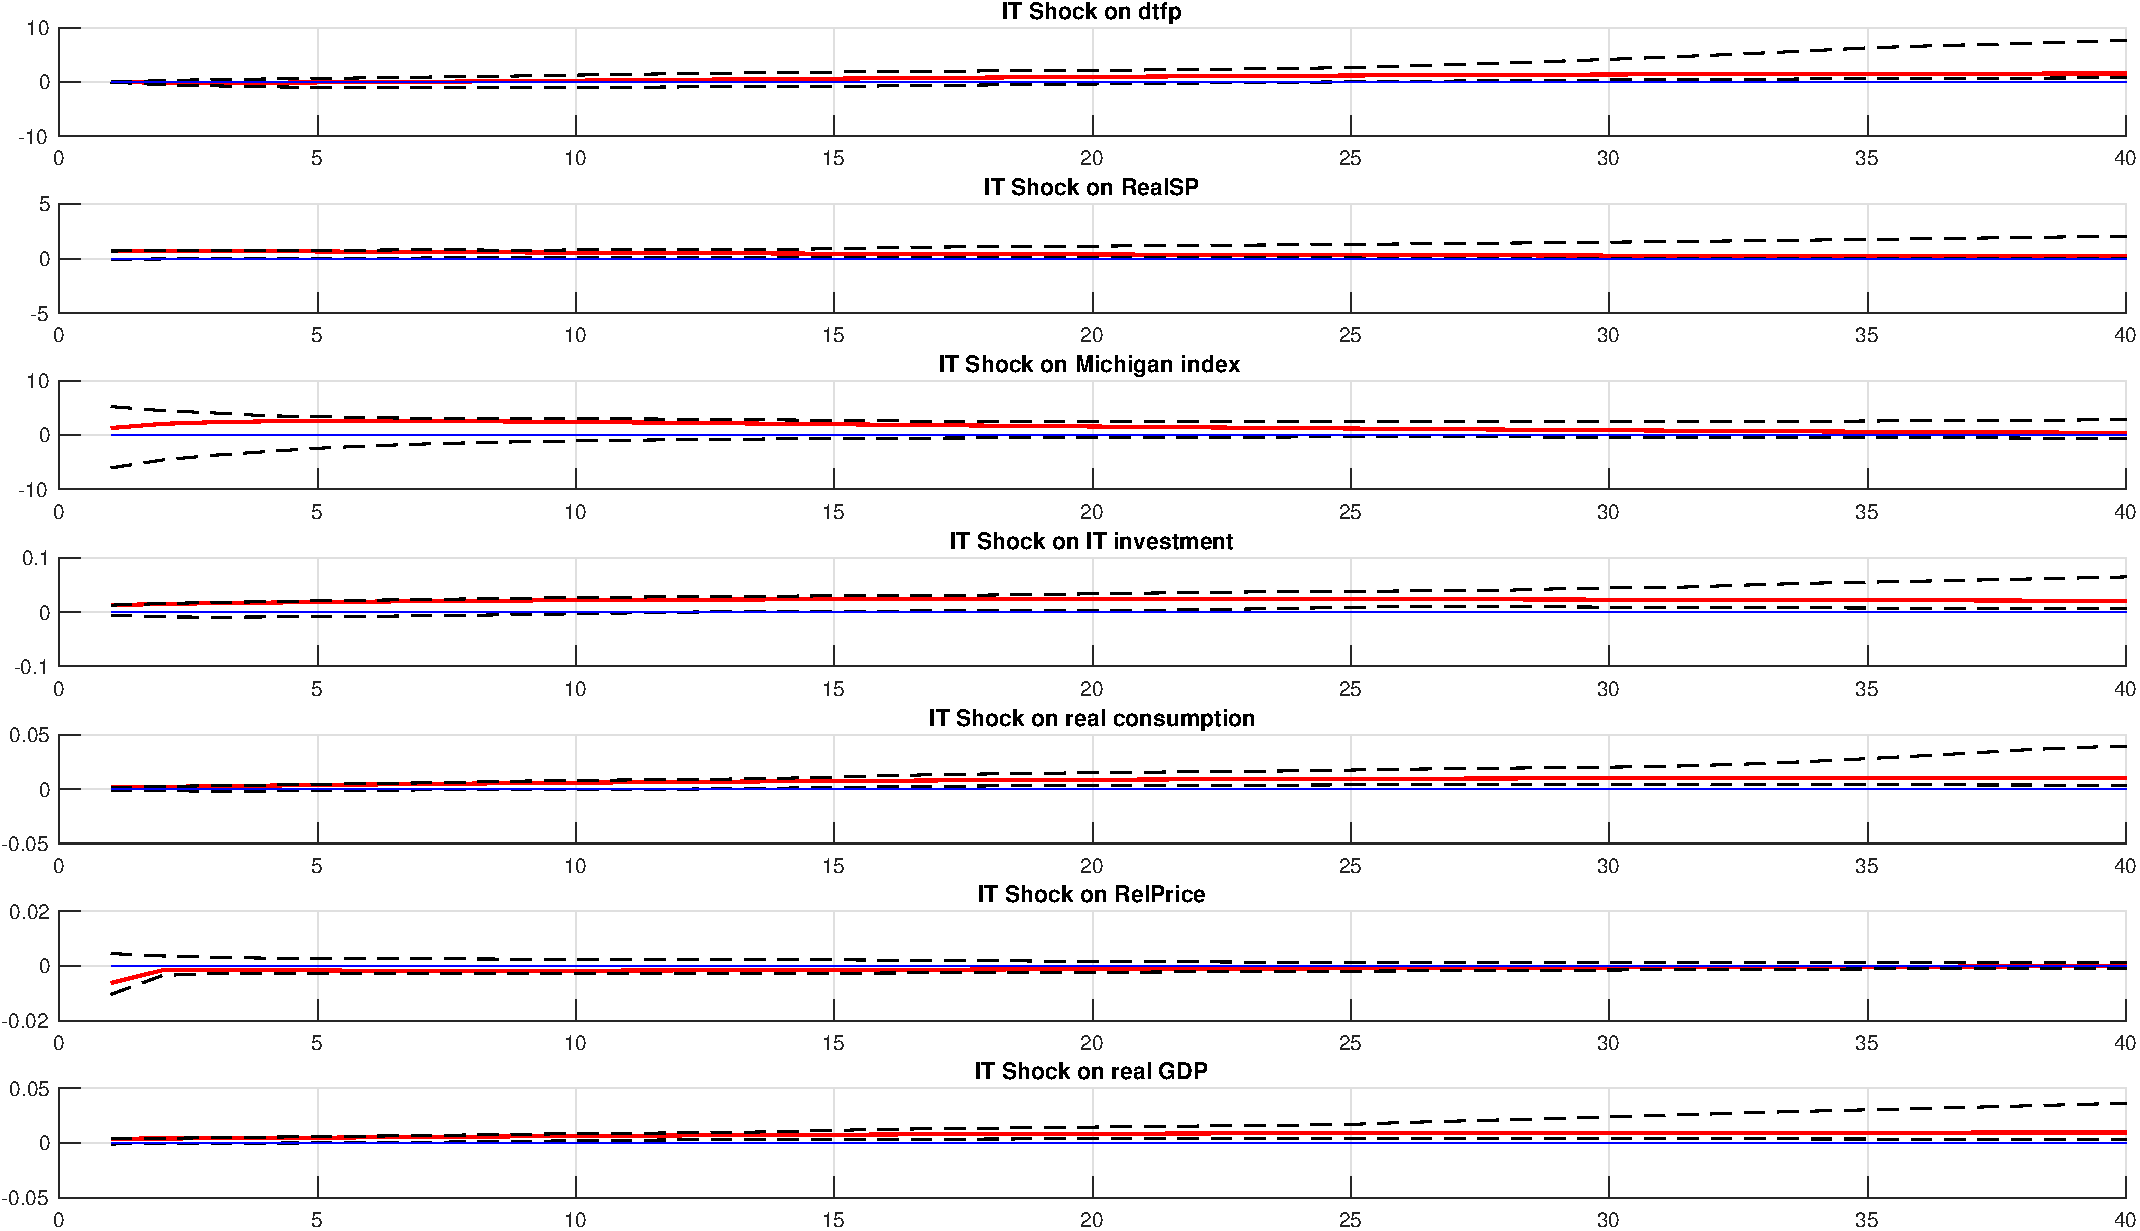
\includegraphics[width=8.5cm]{\ourFigPath Figures/fig_IT_Shock_Ryan_two_stepsID_26-Nov-2017_09_36_11}}
\end{figure}

\

I wanted to do this to see if in the previous spec, it was adding SP500 that made things nicer or if it was removing GDP. Clearly, if you keep GDP in, things aren't so nice anymore, but they're not too bad. Things don't move so much anymore; it seems like we have too many variables for the VAR to contain. At the same time, overall they move in the right directions. 

%%%%%%%%
%SP500 instead of Mich
\newpage
	\subsection{Relative prices LR horizon 8, adding SP 500 instead of Mich}
	\noindent one lag, LR hor = 8, adding real stock prices 500 instead of Mich, leaving in GDP, with relative price; only 30 bootstrap
	
	\
	
	
	\begin{small}
	\begin{tabular}{lccc}
	\hline
		& News & IT & Total \\
		\hline
		Share of TFP FEV explained & 0.4 & 0.4 & 0.8 \\
		\hline
	\end{tabular}
\end{small}

	
	\begin{figure}[h!]
\centering
\subfigure[News]{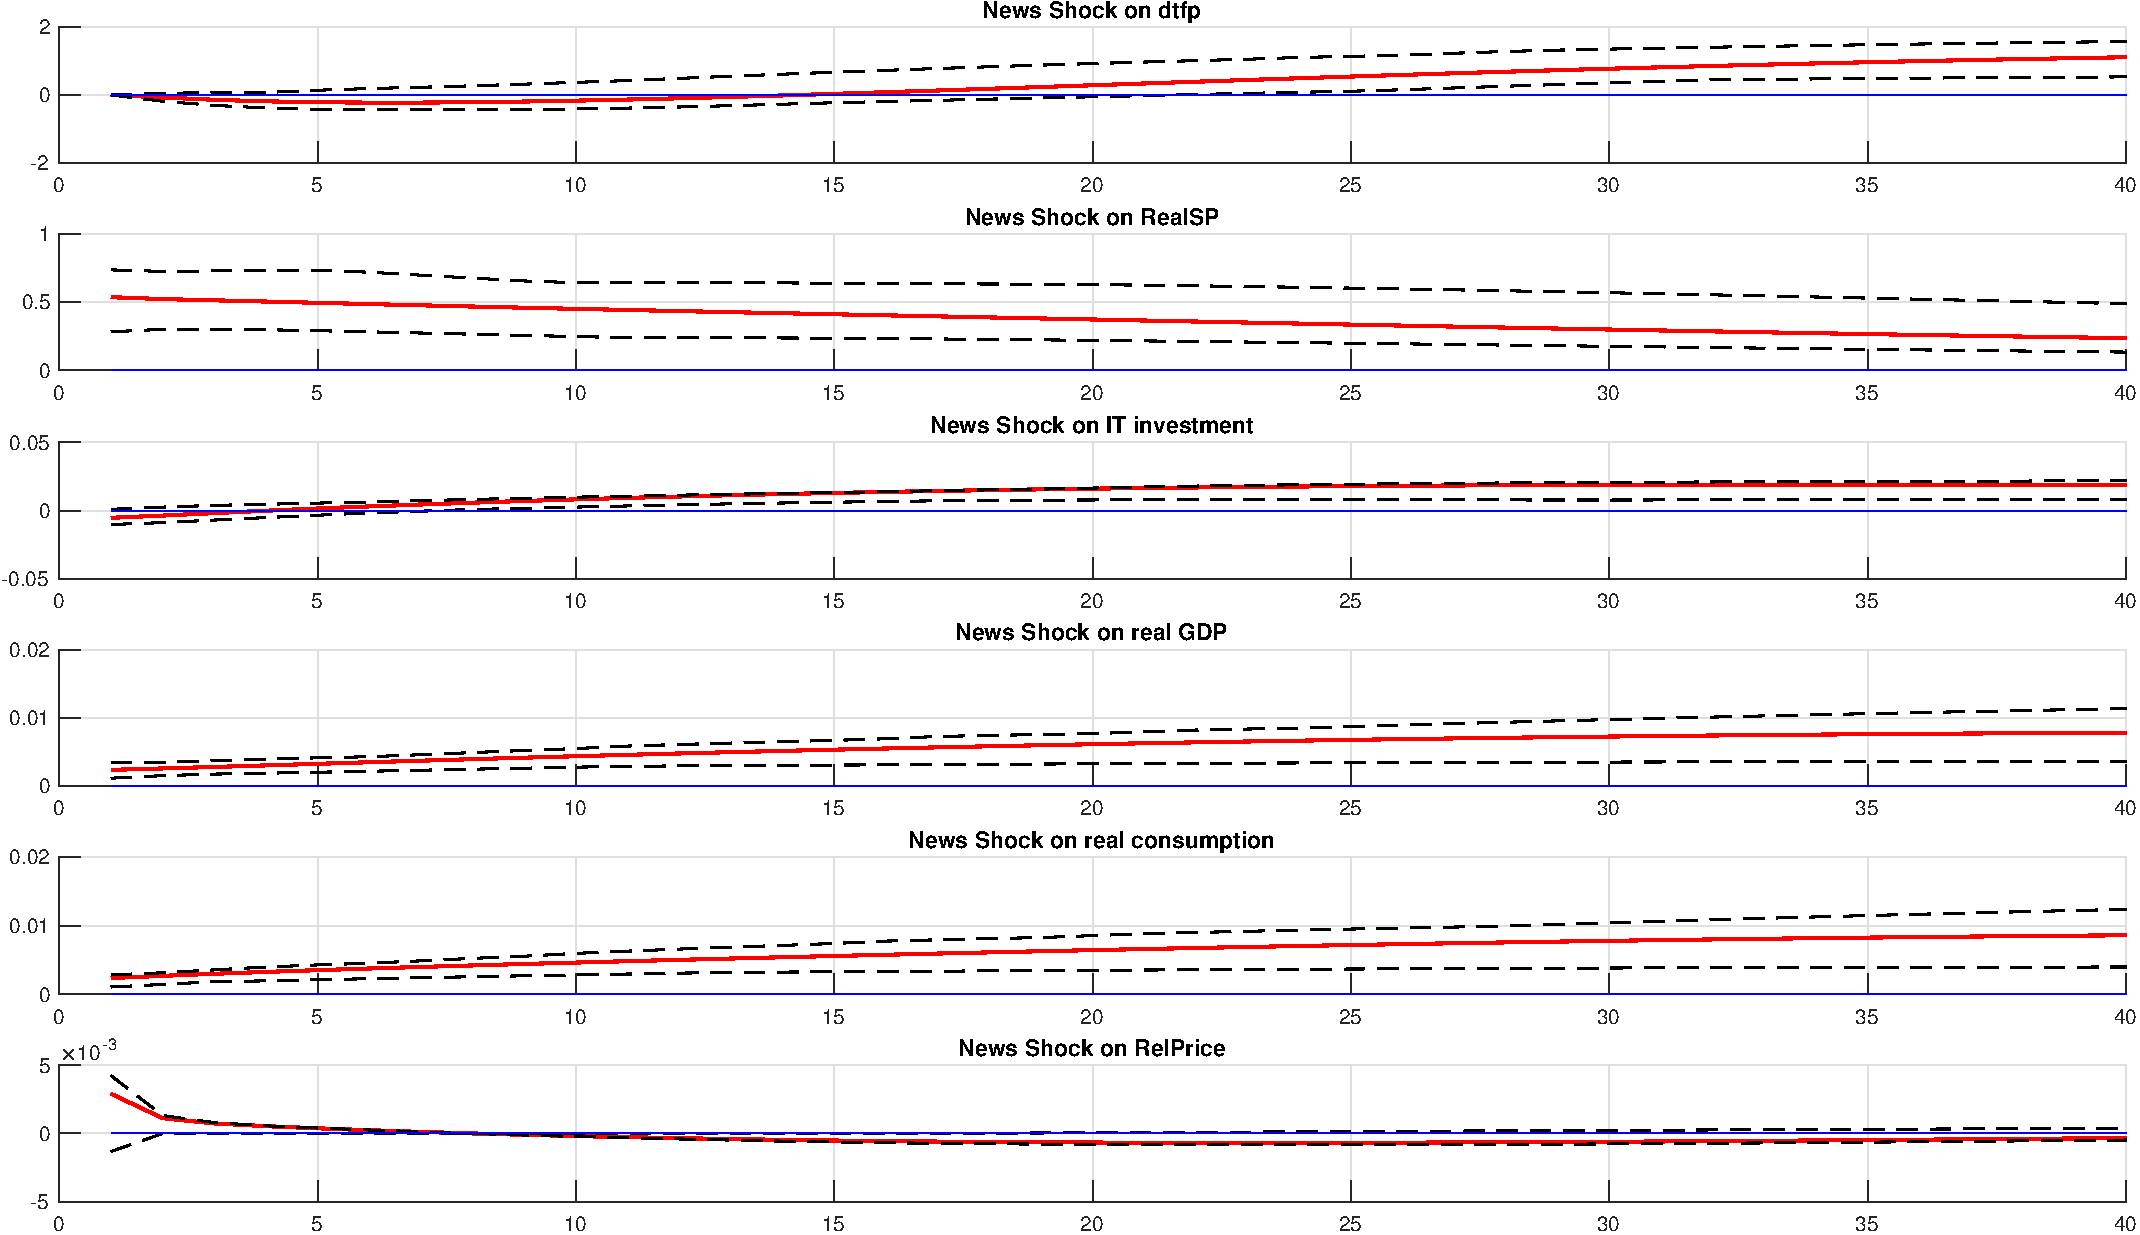
\includegraphics[width=8.5cm]{\ourFigPath Figures/fig_News_Shock_Ryan_two_stepsID_26-Nov-2017_10_02_09}} \hspace{.2in%
} 
\subfigure[IT]{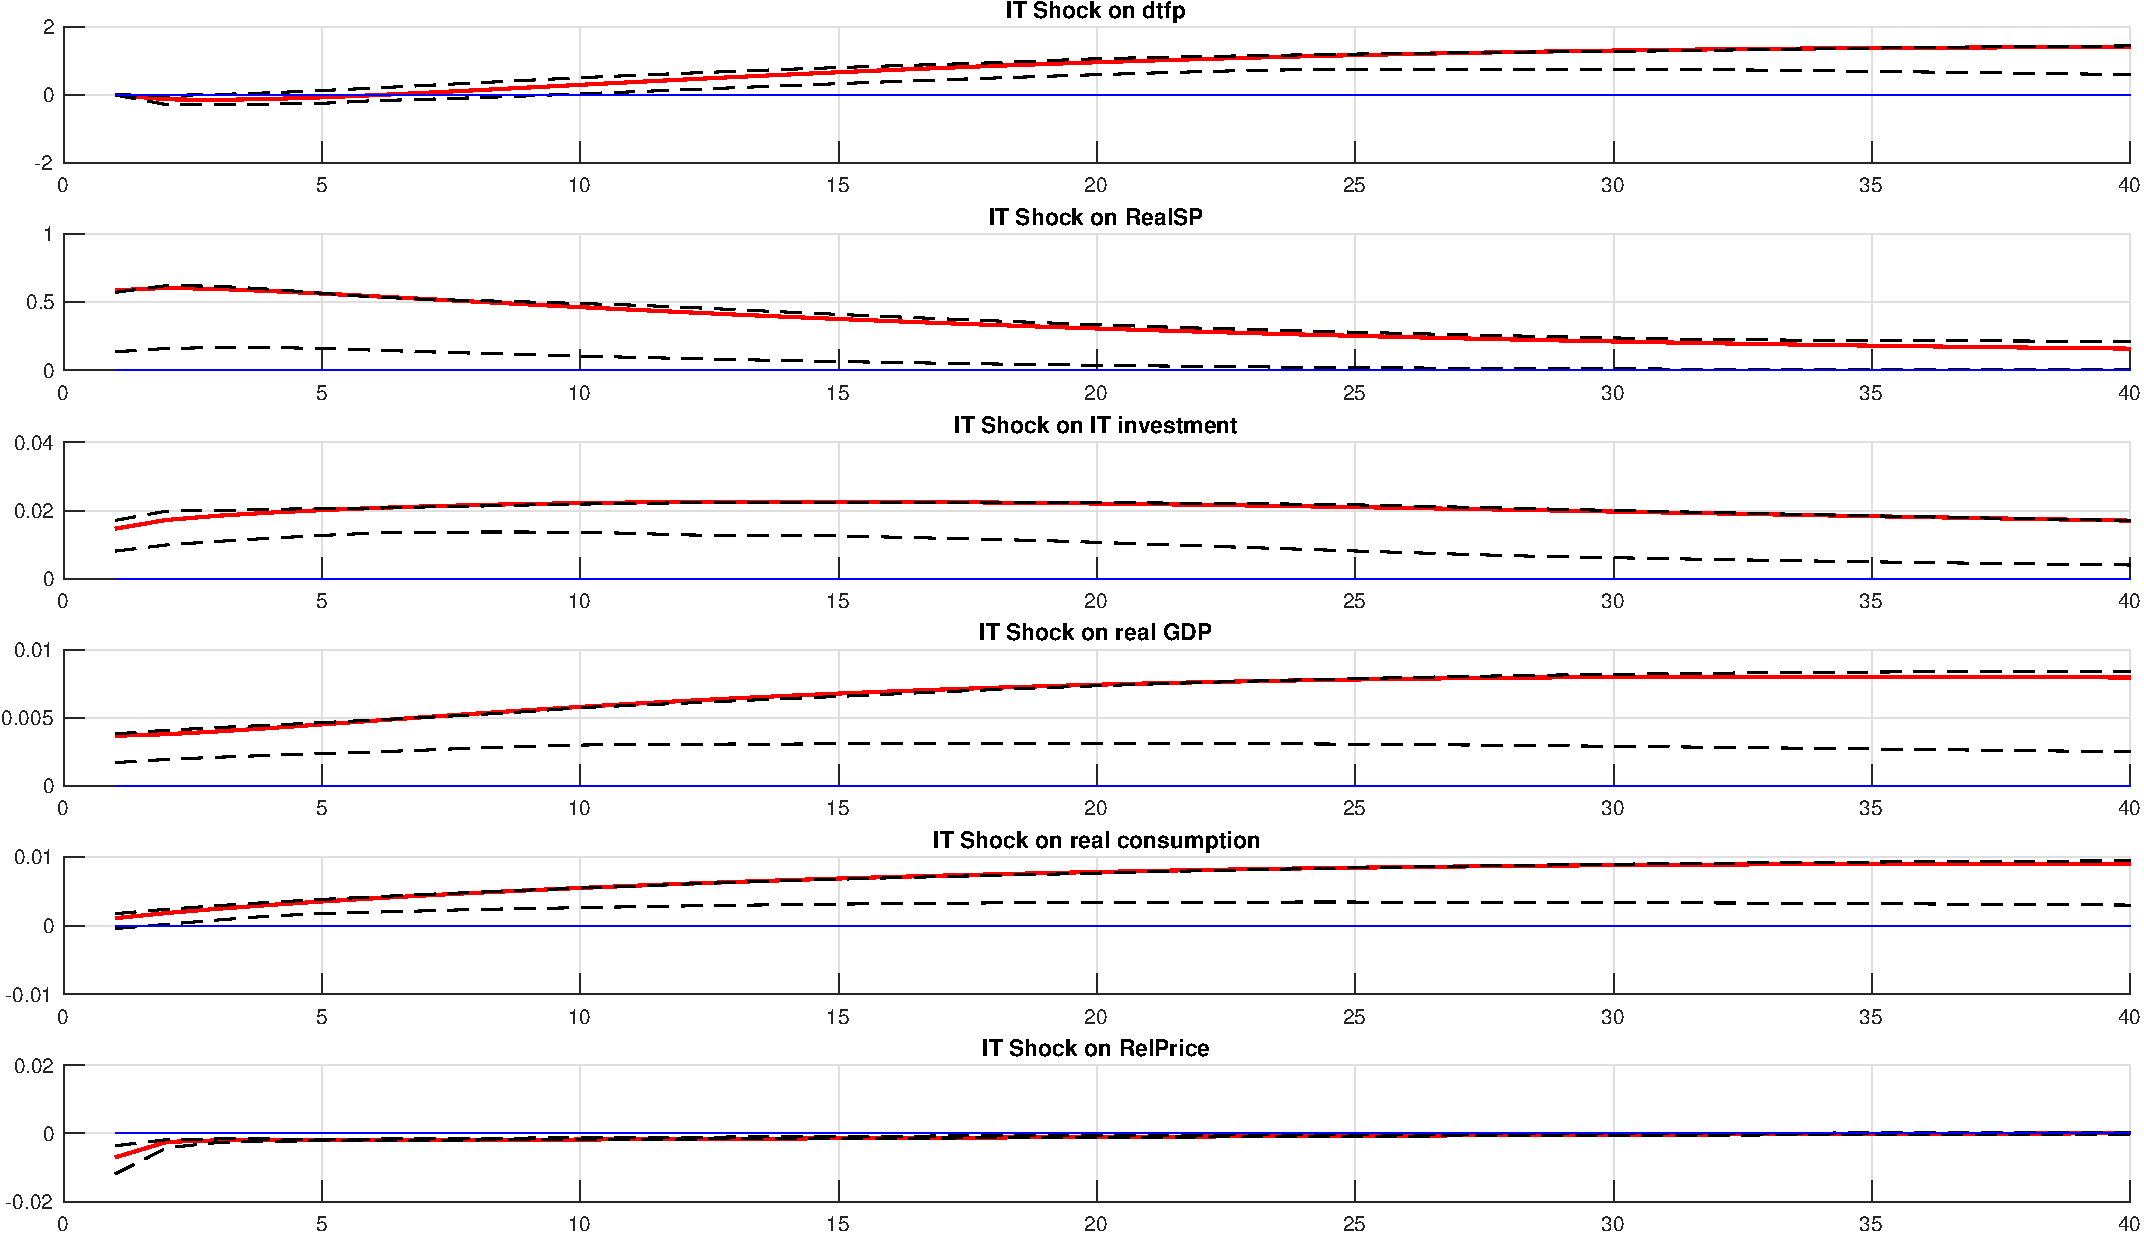
\includegraphics[width=8.5cm]{\ourFigPath Figures/fig_IT_Shock_Ryan_two_stepsID_26-Nov-2017_10_02_14}}
\end{figure}

\

I wanted to do this one to see how well SP500 can replace Mich. Results are fairly in line, that's great, contribution of news and IT is \emph{identical}. VERY nice!
%%%%%%%%
%two lags (back to LR hor = 8, back to no SP500 i.e. default setup)
\newpage
	\subsection{Default spec, 2 lags}
	\noindent two lags, LR hor = 8, Mich is back, with relative price; only 30 bootstrap
	
	\
	
	
	\begin{small}
	\begin{tabular}{lccc}
	\hline
		& News & IT & Total \\
		\hline
		Share of TFP FEV explained & 0.2 & 0.6 & 0.8 \\
		\hline
	\end{tabular}
\end{small}

	
	\begin{figure}[h!]
\centering
\subfigure[News]{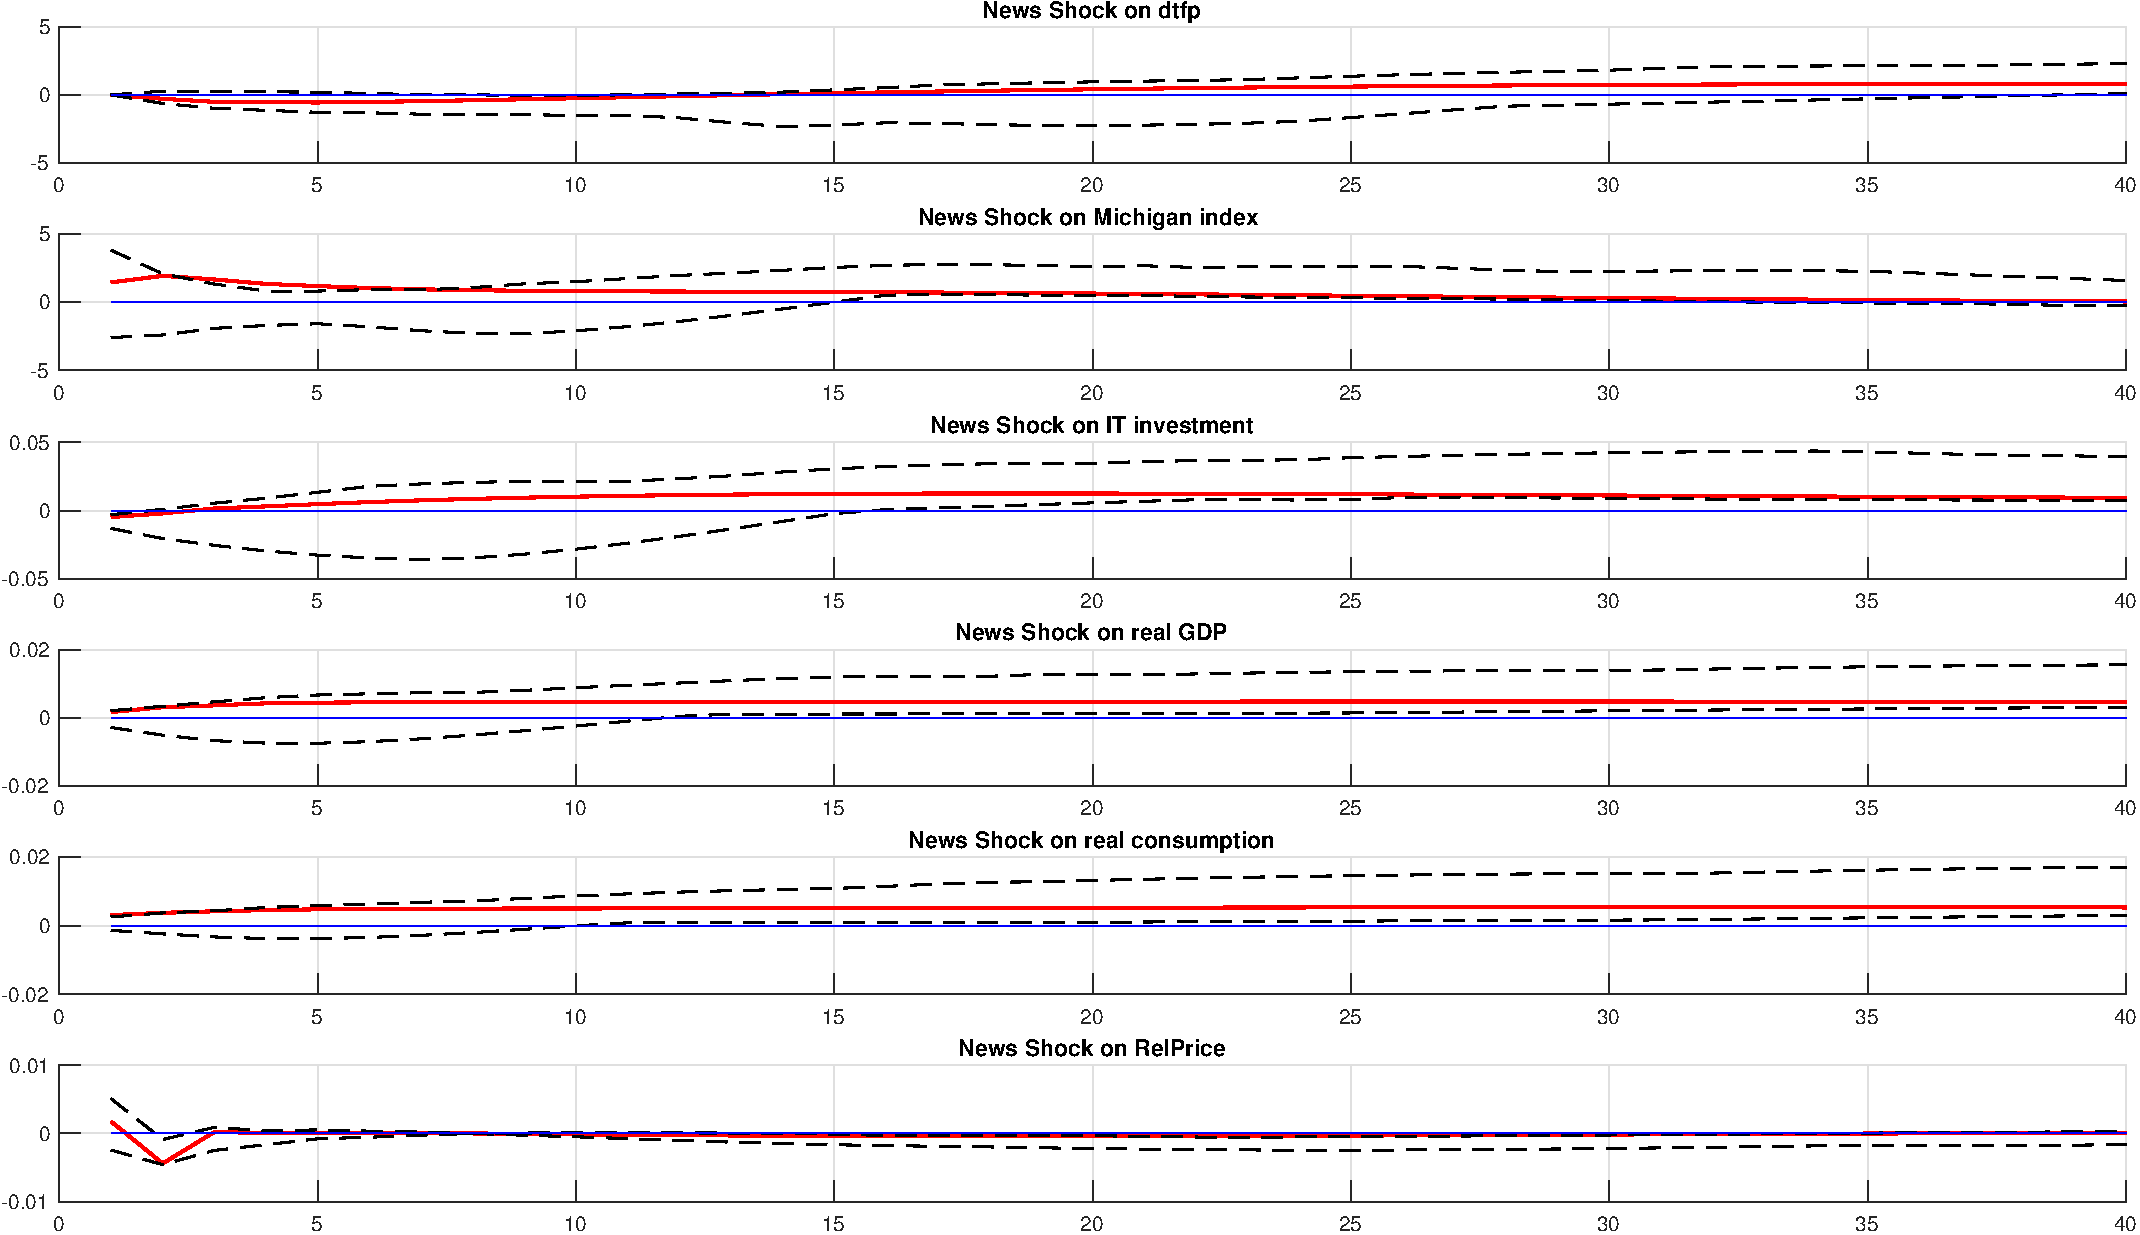
\includegraphics[width=8.5cm]{\ourFigPath Figures/fig_News_Shock_Ryan_two_stepsID_26-Nov-2017_10_12_10}} \hspace{.2in%
} 
\subfigure[IT]{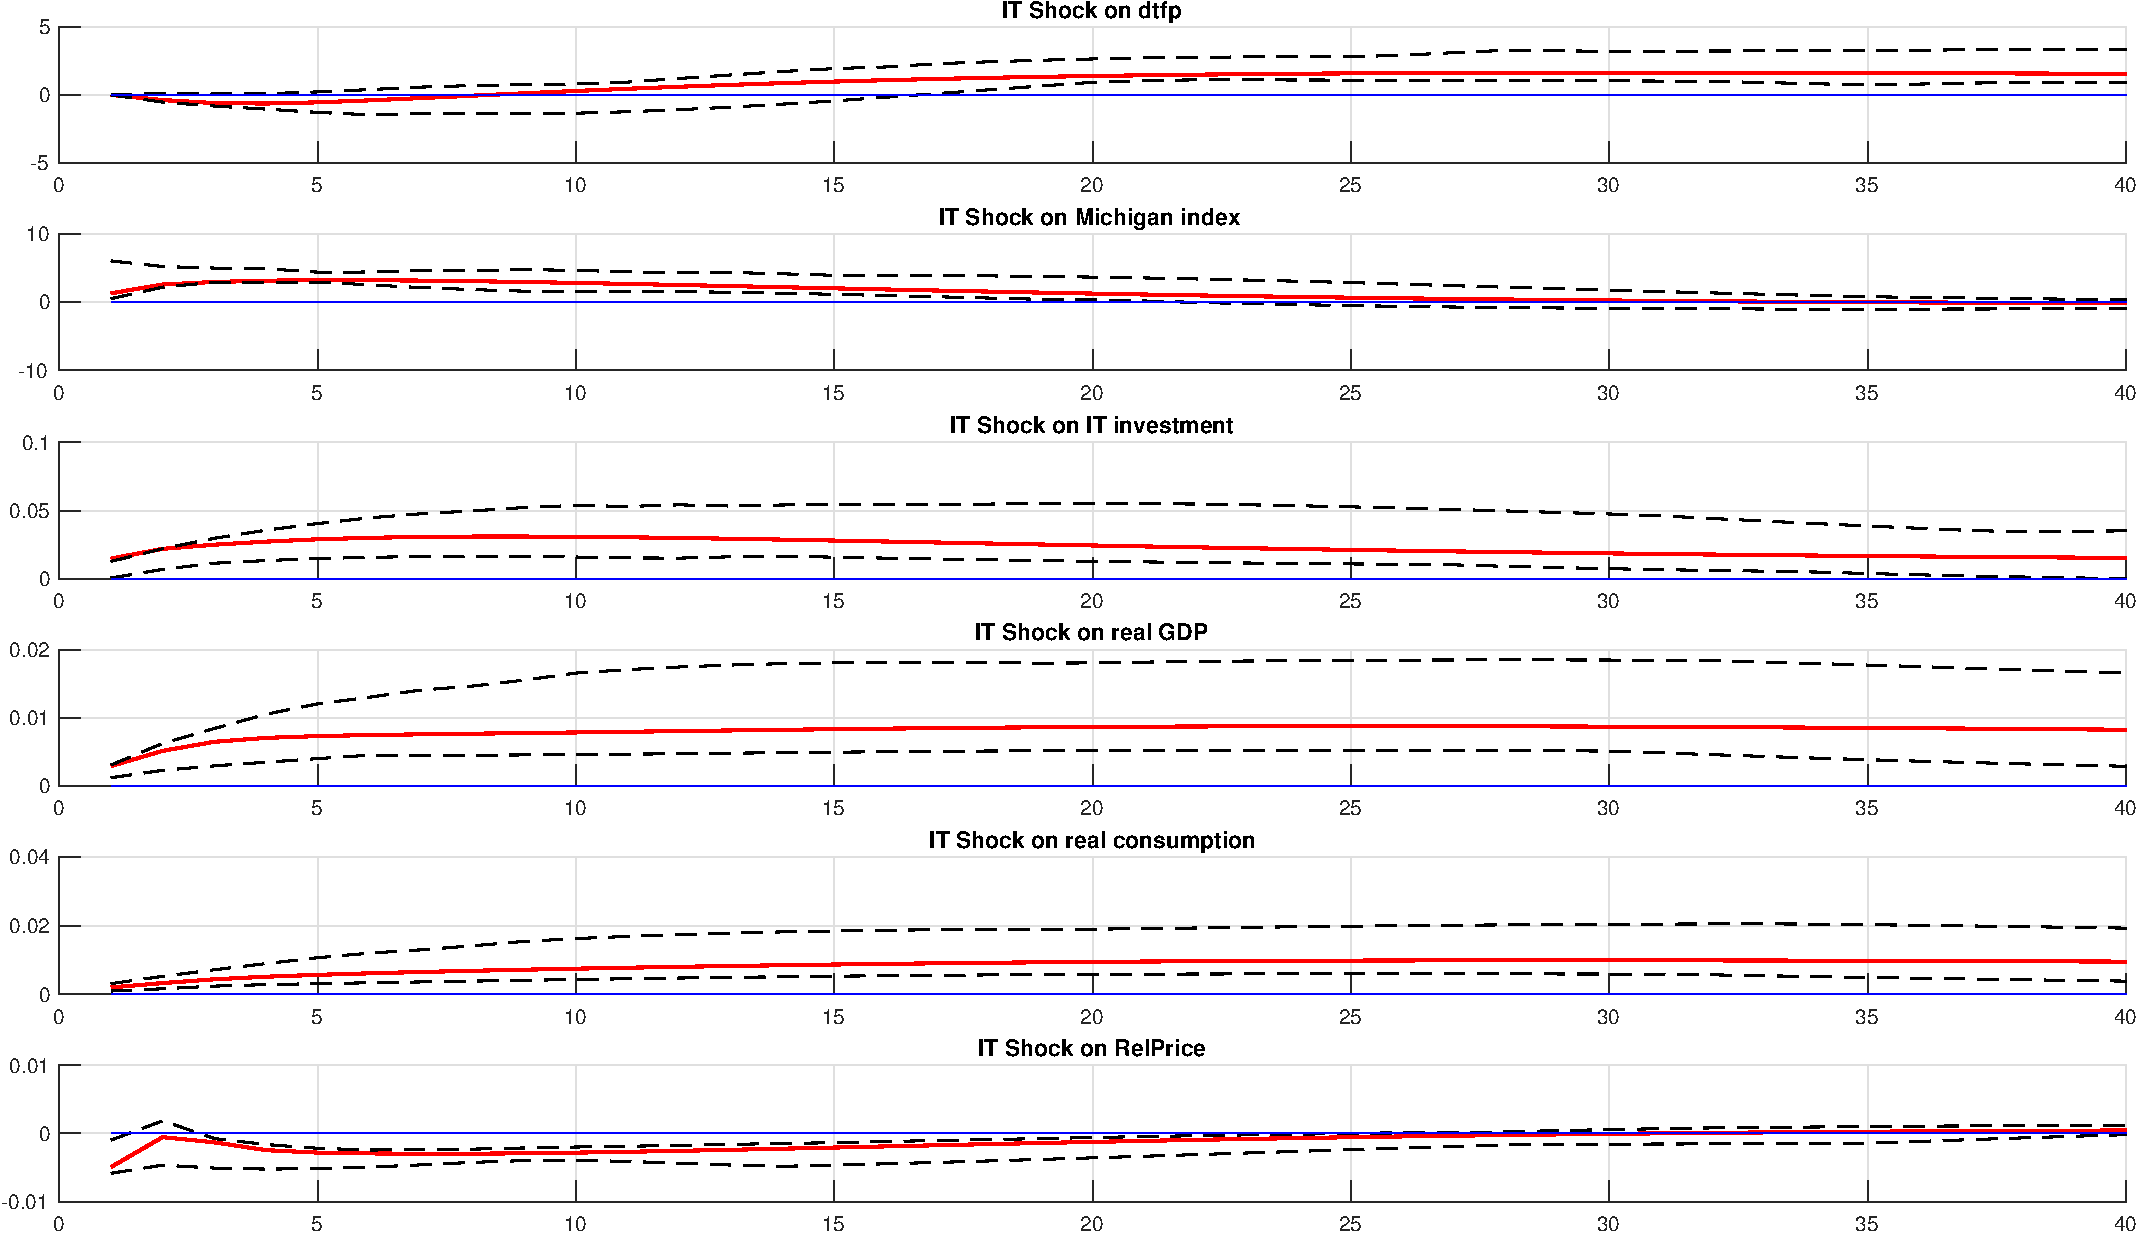
\includegraphics[width=8.5cm]{\ourFigPath Figures/fig_IT_Shock_Ryan_two_stepsID_26-Nov-2017_10_12_14}}
\end{figure}

\
A little too much uncertainty here on the news shock side. Doing this with a 500 bootstrap might make sense. % Running on server, expected to be ready around 16.00



%%%%%%%%
% removing consumption 
\newpage
	\subsection{Default spec, removing consumption}
	\noindent one lag, LR hor = 8, no consumption, with relative price; only 30 bootstrap
	
	\
	
	
	\begin{small}
	\begin{tabular}{lccc}
	\hline
		& News & IT & Total \\
		\hline
		Share of TFP FEV explained & 0.2 & 0.6 & 0.8 \\
		\hline
	\end{tabular}
\end{small}

	
	\begin{figure}[h!]
\centering
\subfigure[News]{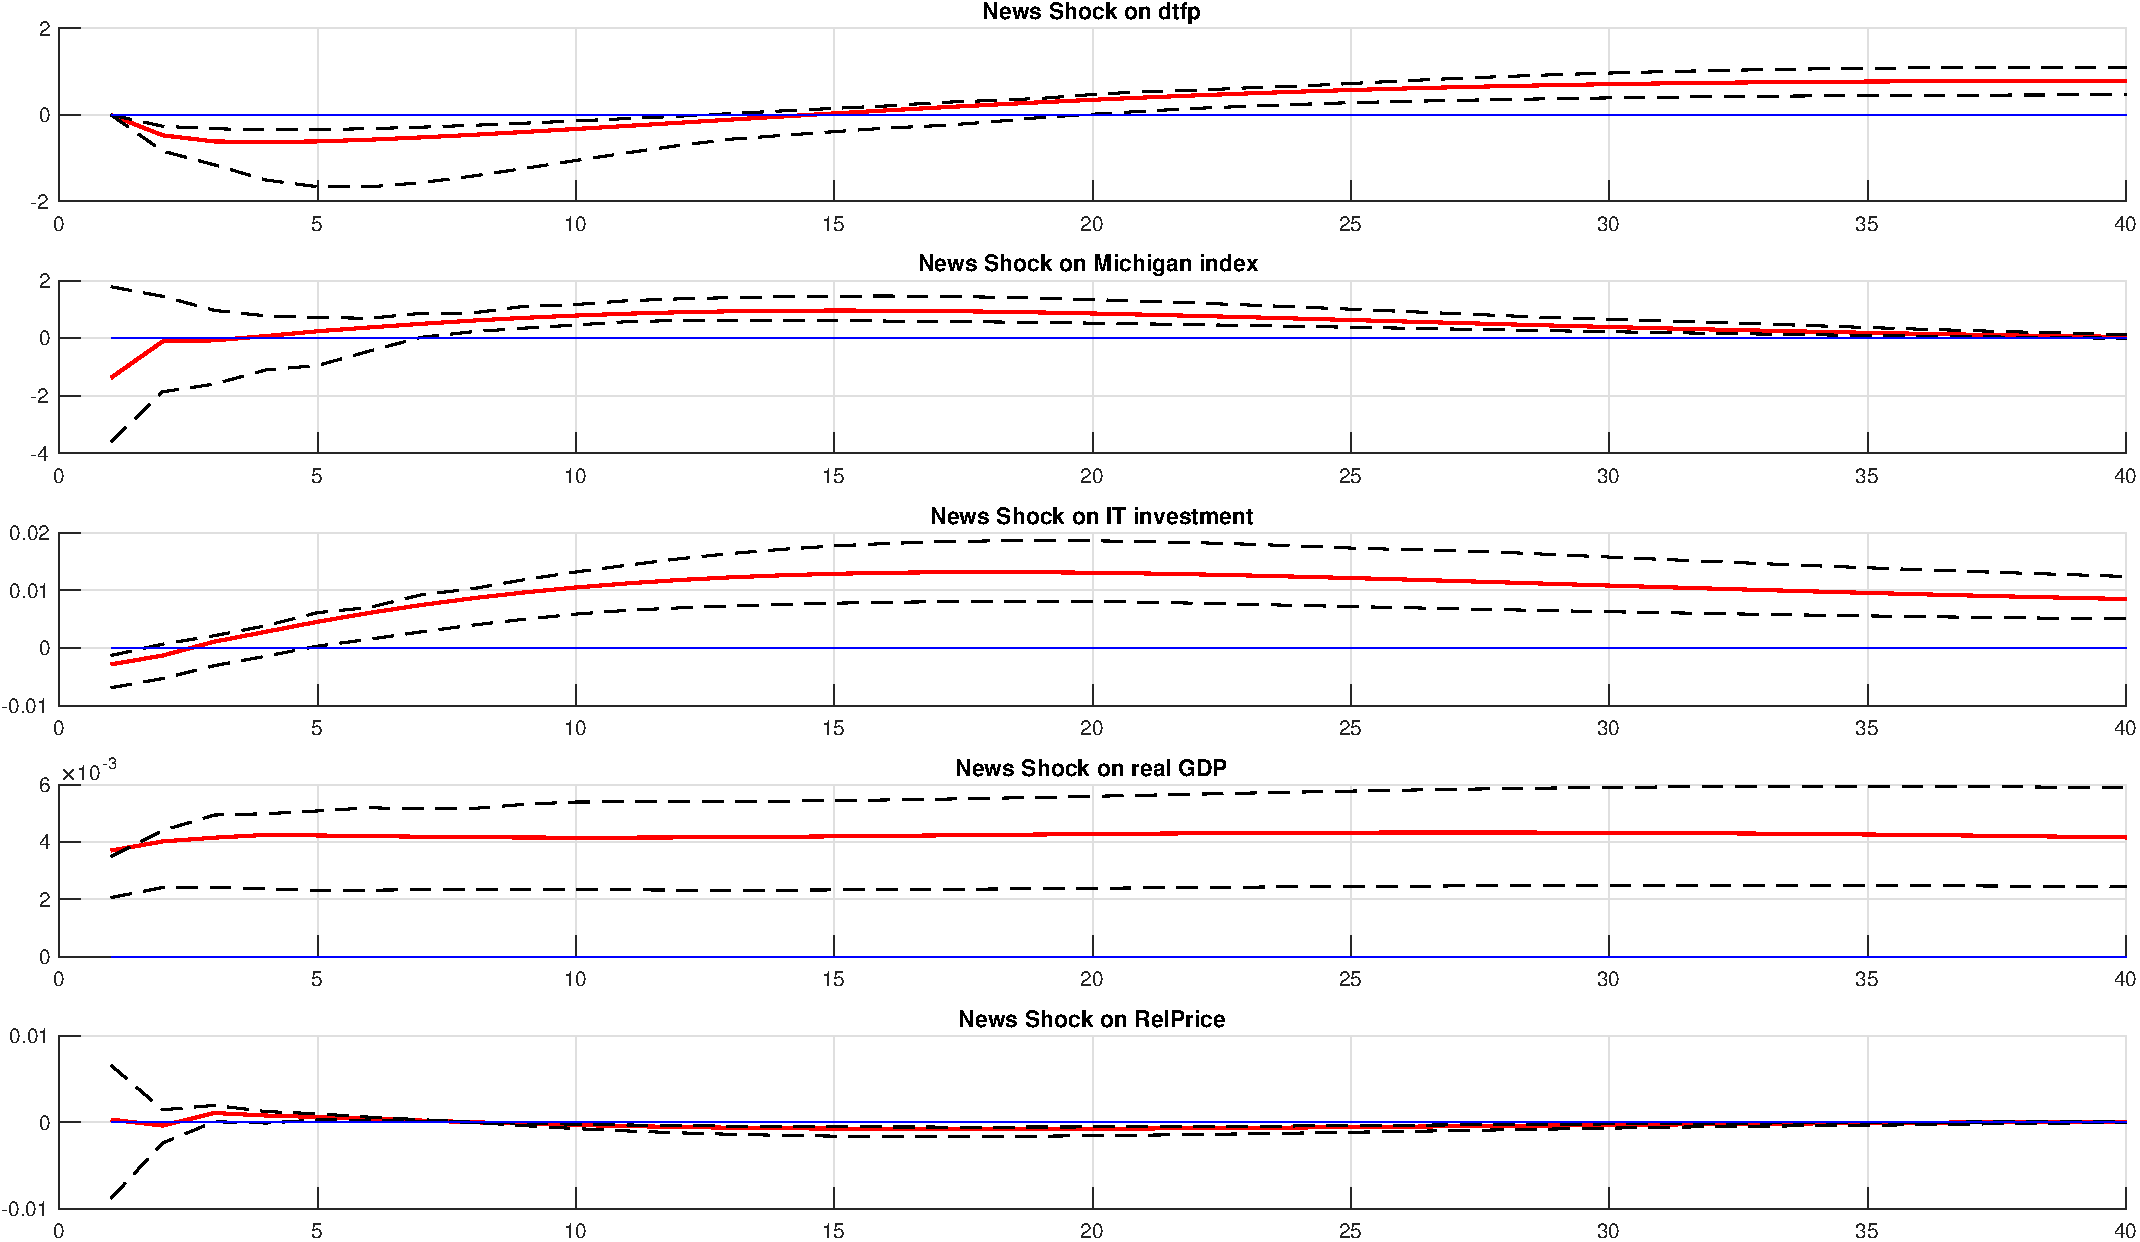
\includegraphics[width=8.5cm]{\ourFigPath Figures/fig_News_Shock_Ryan_two_stepsID_26-Nov-2017_10_24_15}} \hspace{.2in%
} 
\subfigure[IT]{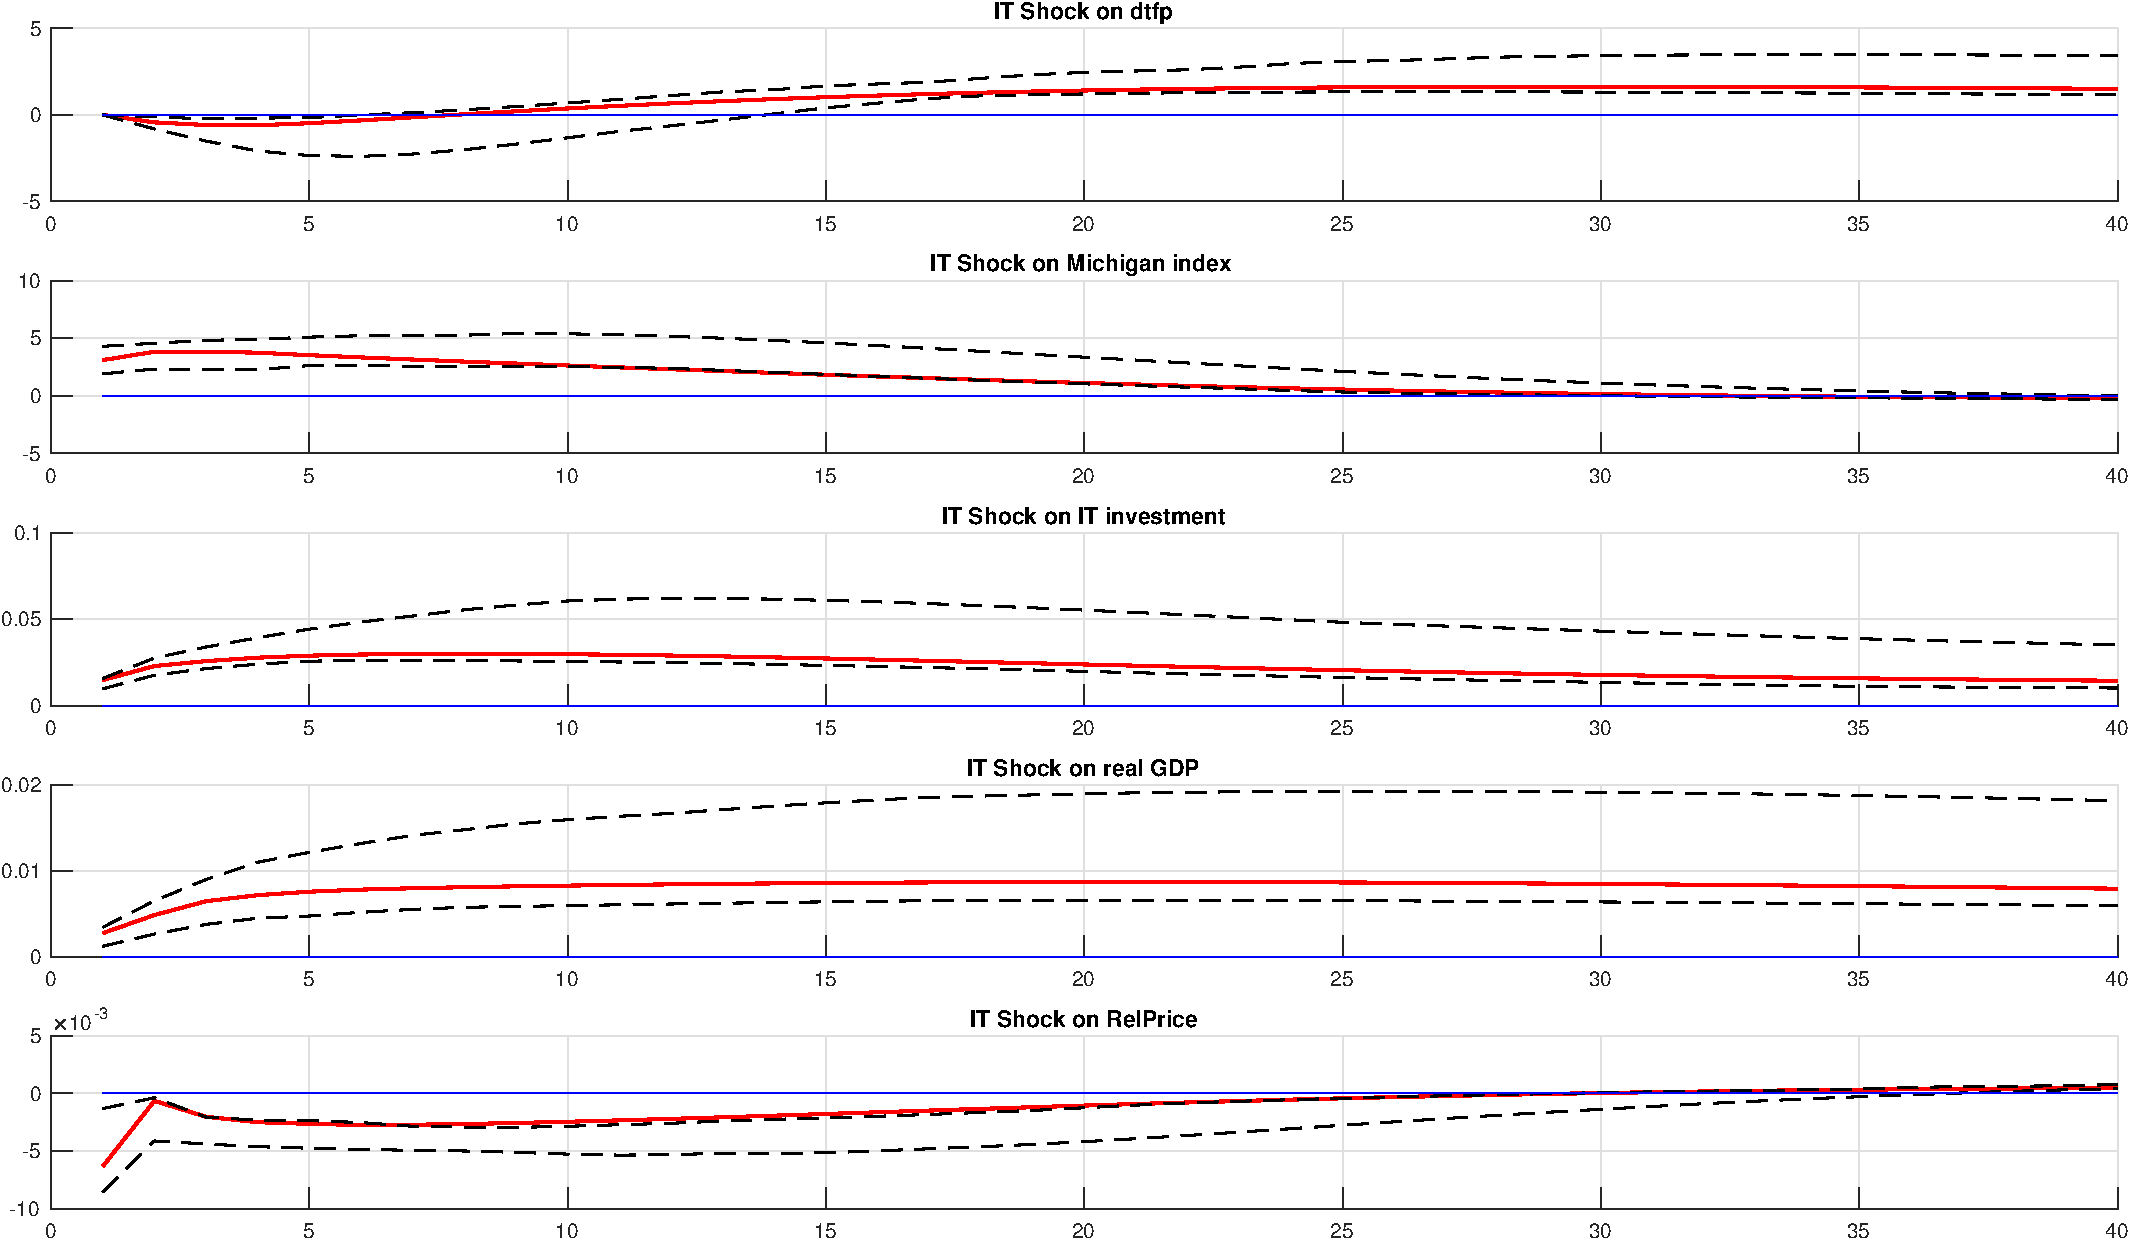
\includegraphics[width=8.5cm]{\ourFigPath Figures/fig_IT_Shock_Ryan_two_stepsID_26-Nov-2017_10_24_19}}
\end{figure}

\

Not too bad, but wiggly - strangely enough, something seems to be missing.

%%%%%%%%
% adding hours 
\newpage
	\subsection{Default spec, adding hours}
	\noindent one lag, LR hor = 8, adding hours, with relative price; only 30 bootstrap
	
	\
	
	
	\begin{small}
	\begin{tabular}{lccc}
	\hline
		& News & IT & Total \\
		\hline
		Share of TFP FEV explained & 0.2 & 0.6 & 0.8 \\
		\hline
	\end{tabular}
\end{small}

	
	\begin{figure}[h!]
\centering
\subfigure[News]{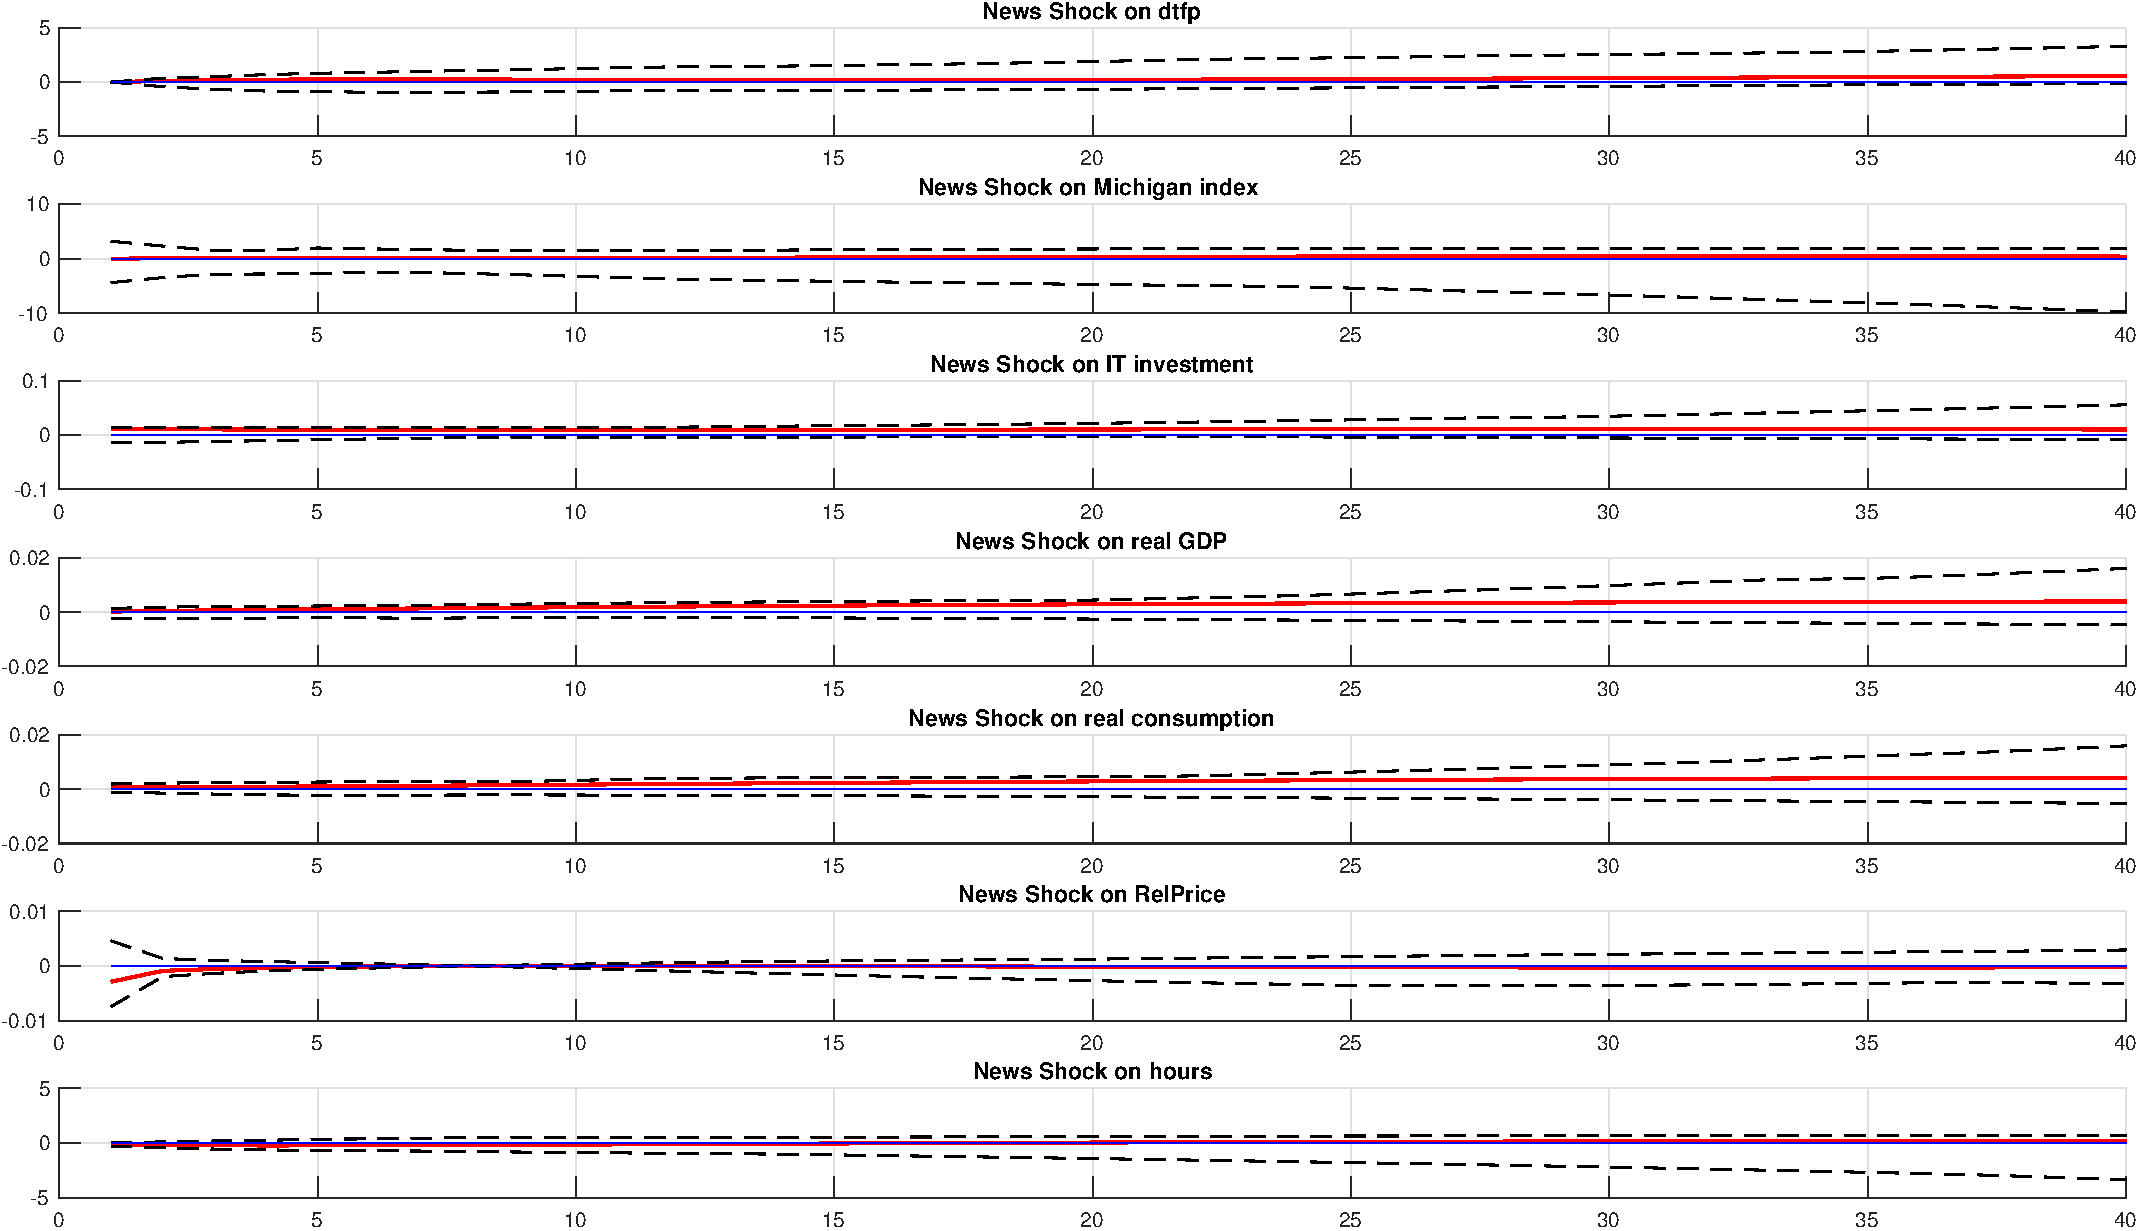
\includegraphics[width=8.5cm]{\ourFigPath Figures/fig_News_Shock_Ryan_two_stepsID_26-Nov-2017_10_43_48}} \hspace{.2in%
} 
\subfigure[IT]{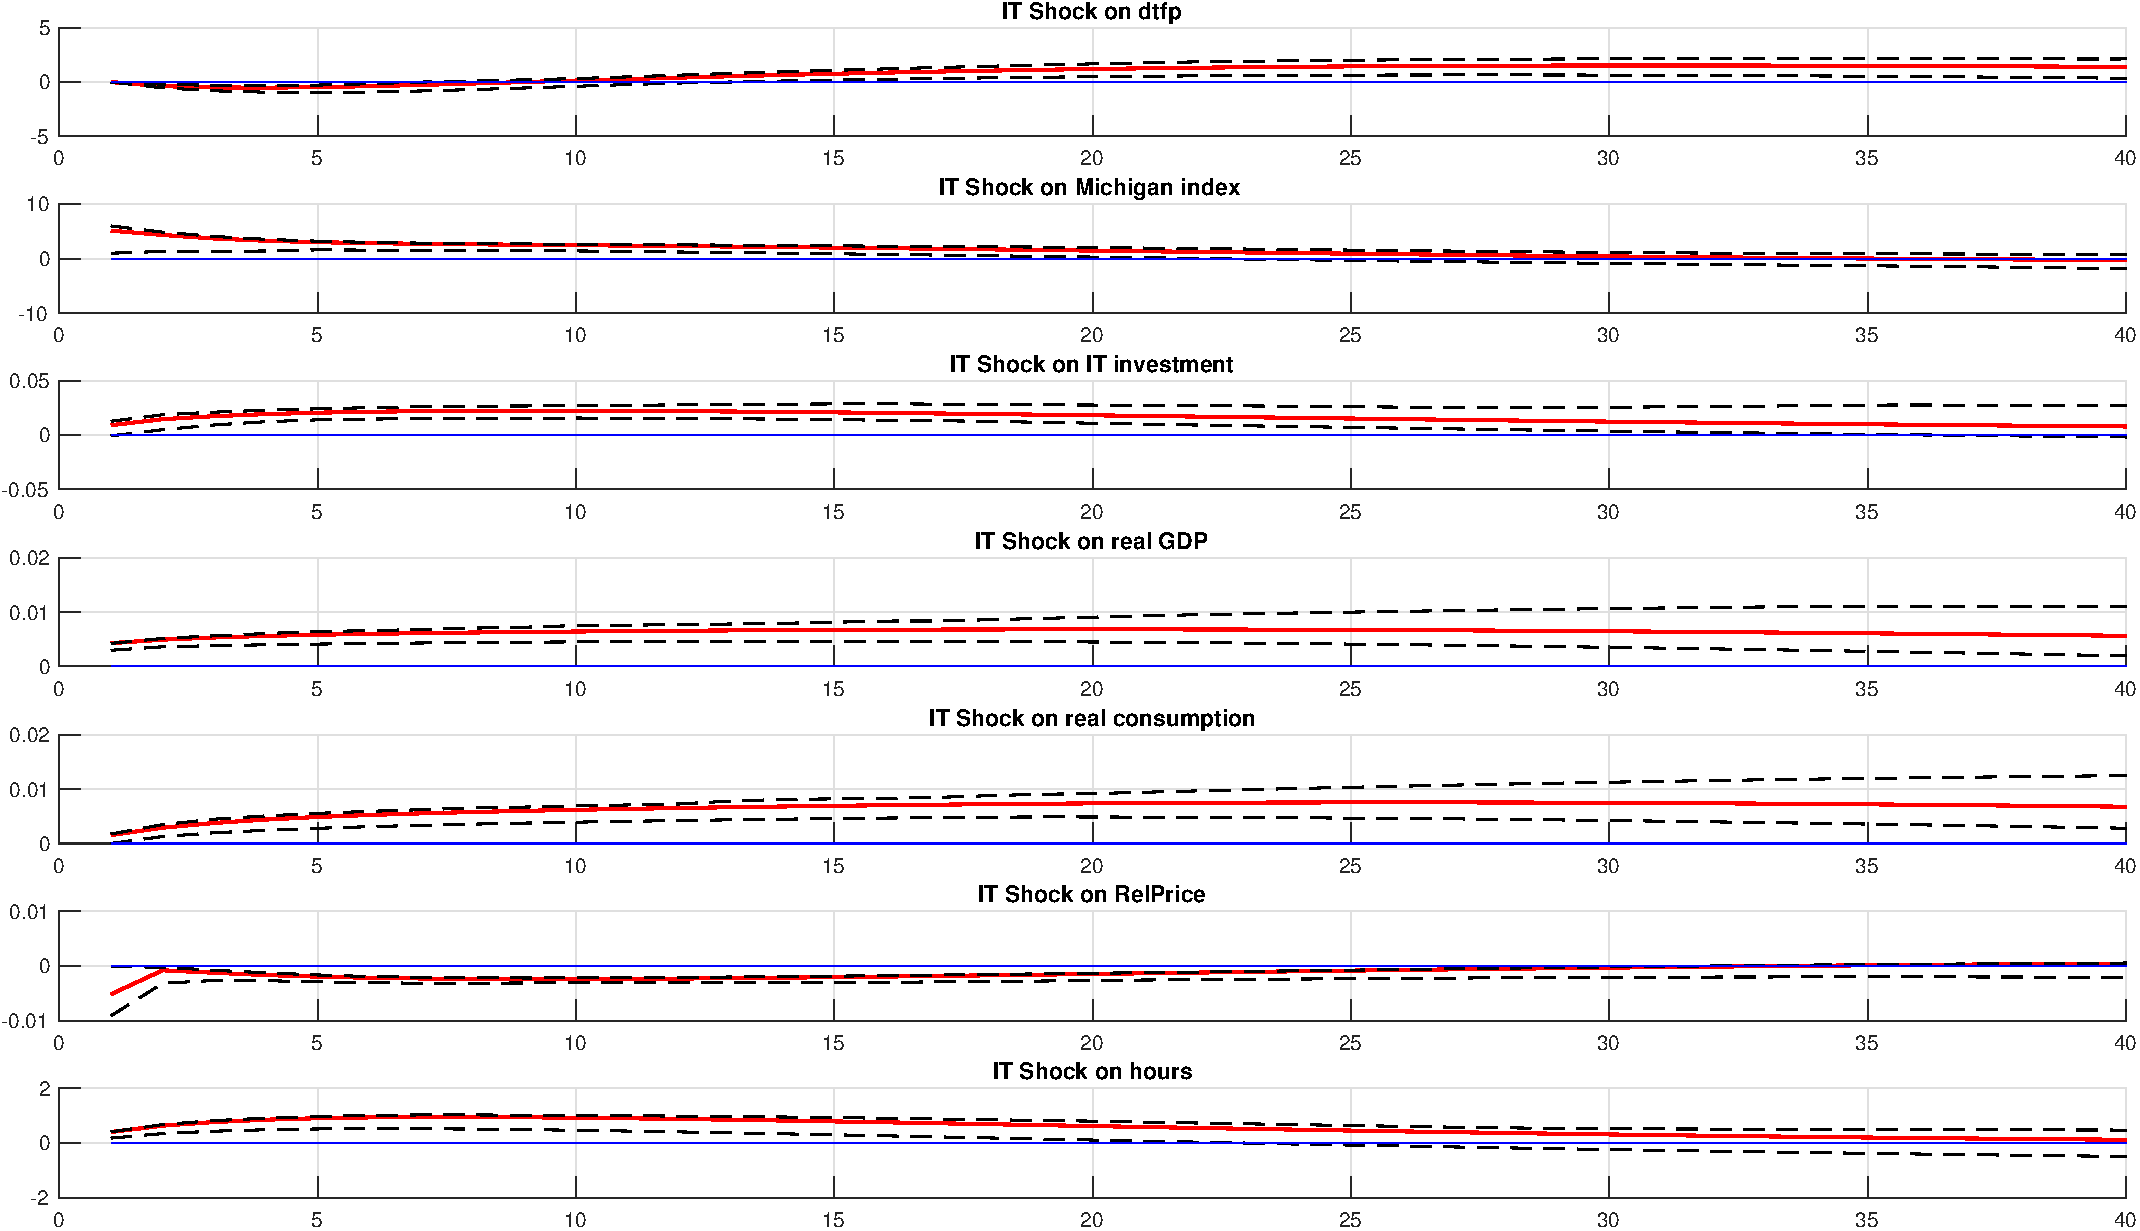
\includegraphics[width=8.5cm]{\ourFigPath Figures/fig_IT_Shock_Ryan_two_stepsID_26-Nov-2017_10_43_51}}
\end{figure}

\
As usual, it screws up the news shock, leaving the IT shock very nice. 


%%%%%%%%
% and/or adding investment 

%%%%%%%%
% Capital prices instead of relative prices
\newpage
\subsection{Capital prices LR horizon 8}
\noindent Time it took, for 500 bootstrap, Mac: 12 min

\noindent  Time it took, for 500 bootstrap, server (w/o parpool): 30 min


\noindent  'News'       'IT'        'Total' 

\noindent  '0.40843'    '0.23982'    '0.64824'


\begin{small}
	\begin{tabular}{lccc}
	\hline
		& News & IT & Total \\
		\hline
		Share of TFP FEV explained & 0.4 & 0.2 & 0.6 \\
		\hline
	\end{tabular}
\end{small}


\begin{figure}[h!]
	\centering
	\subfigure[News]{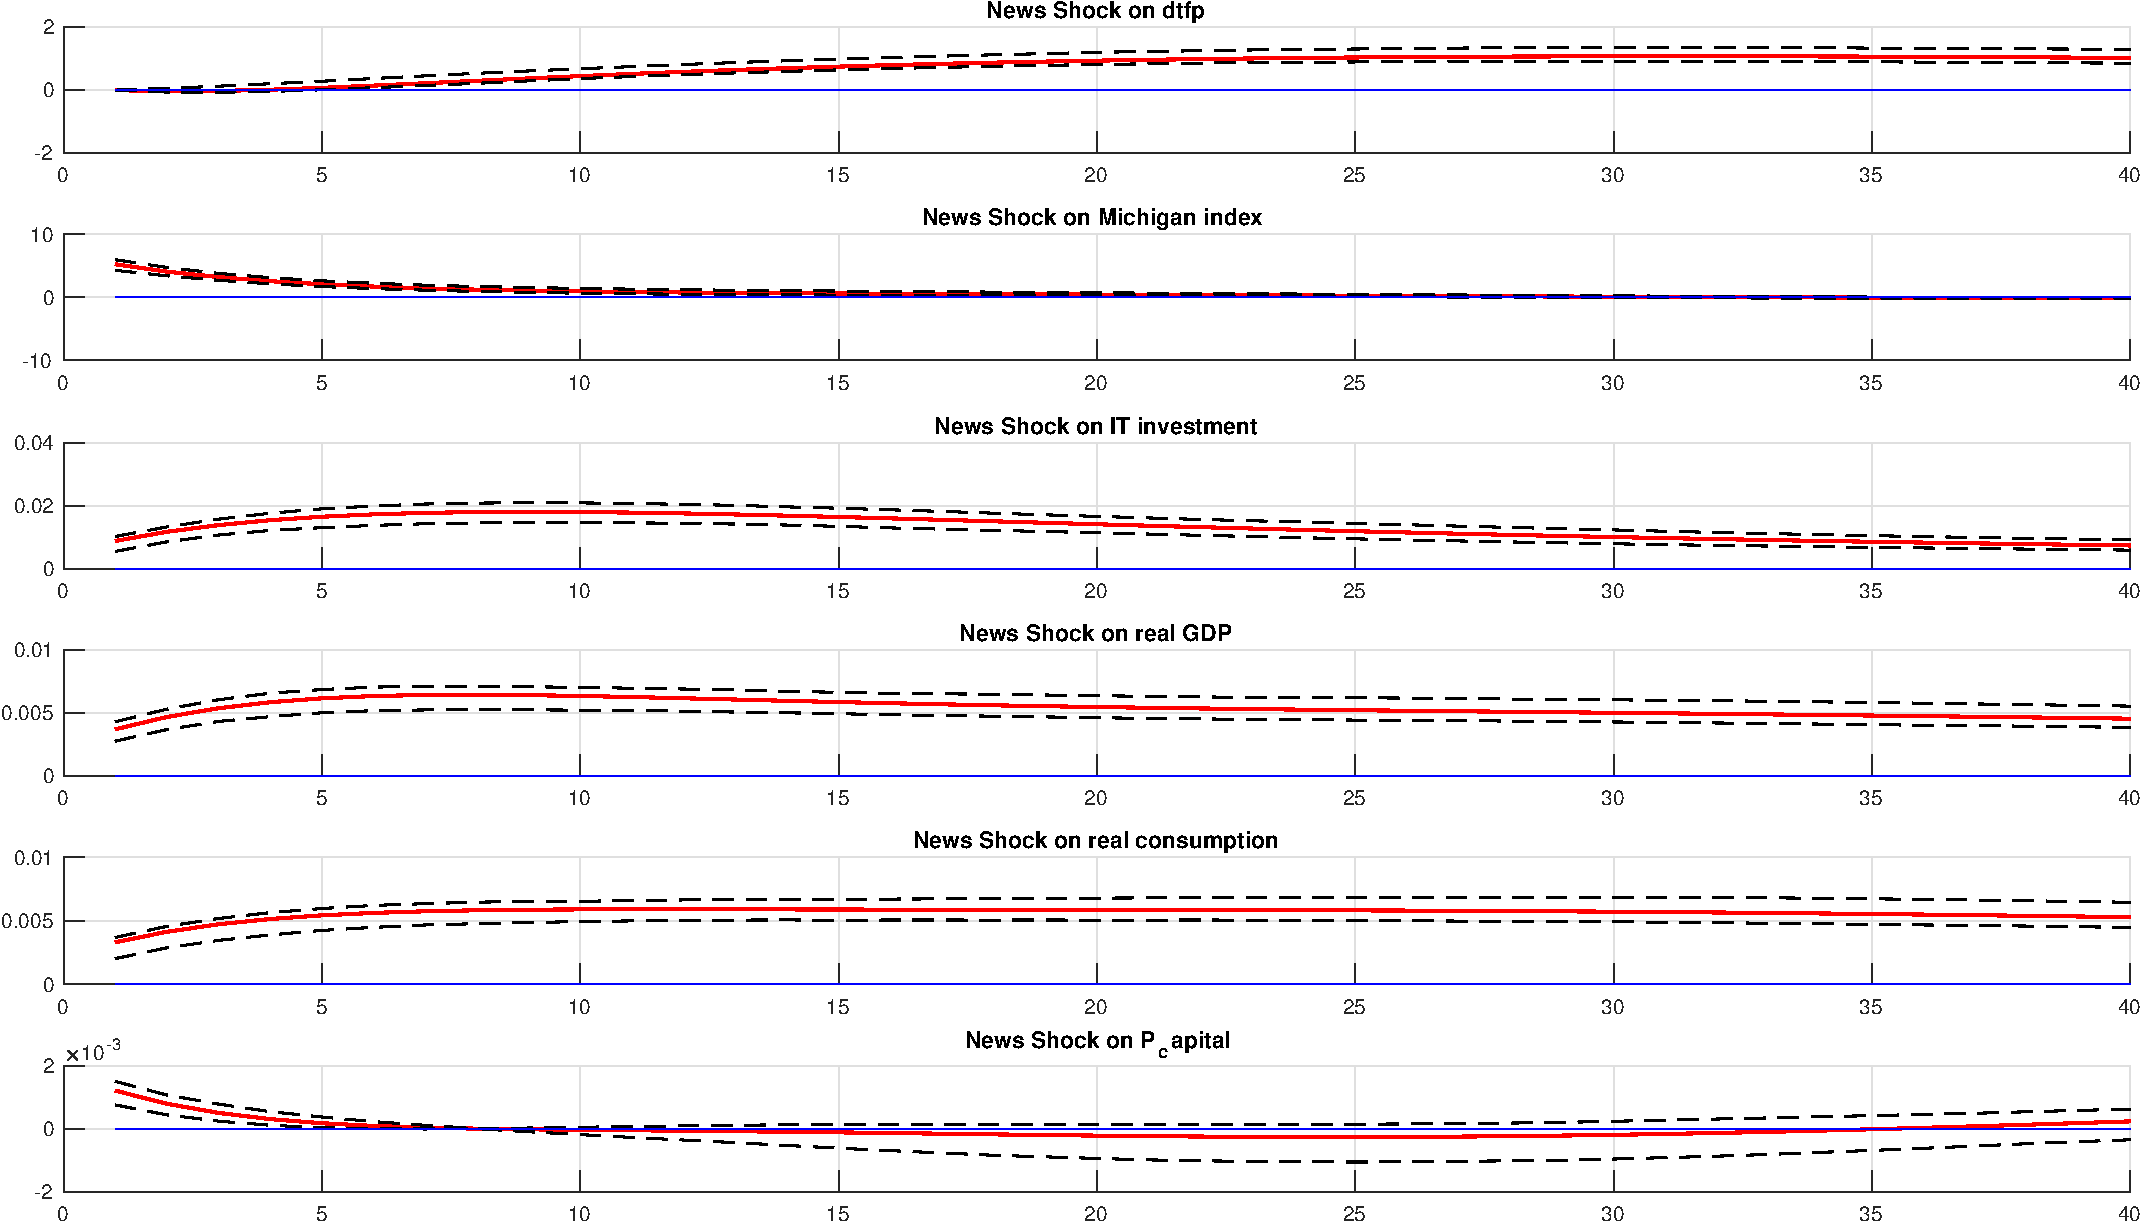
\includegraphics[width=8.5cm]{\ourFigPath Figures/fig_News_Shock_Ryan_two_stepsID_24-Nov-2017_16_17_15}} \hspace{.2in%
	} 
	\subfigure[IT]{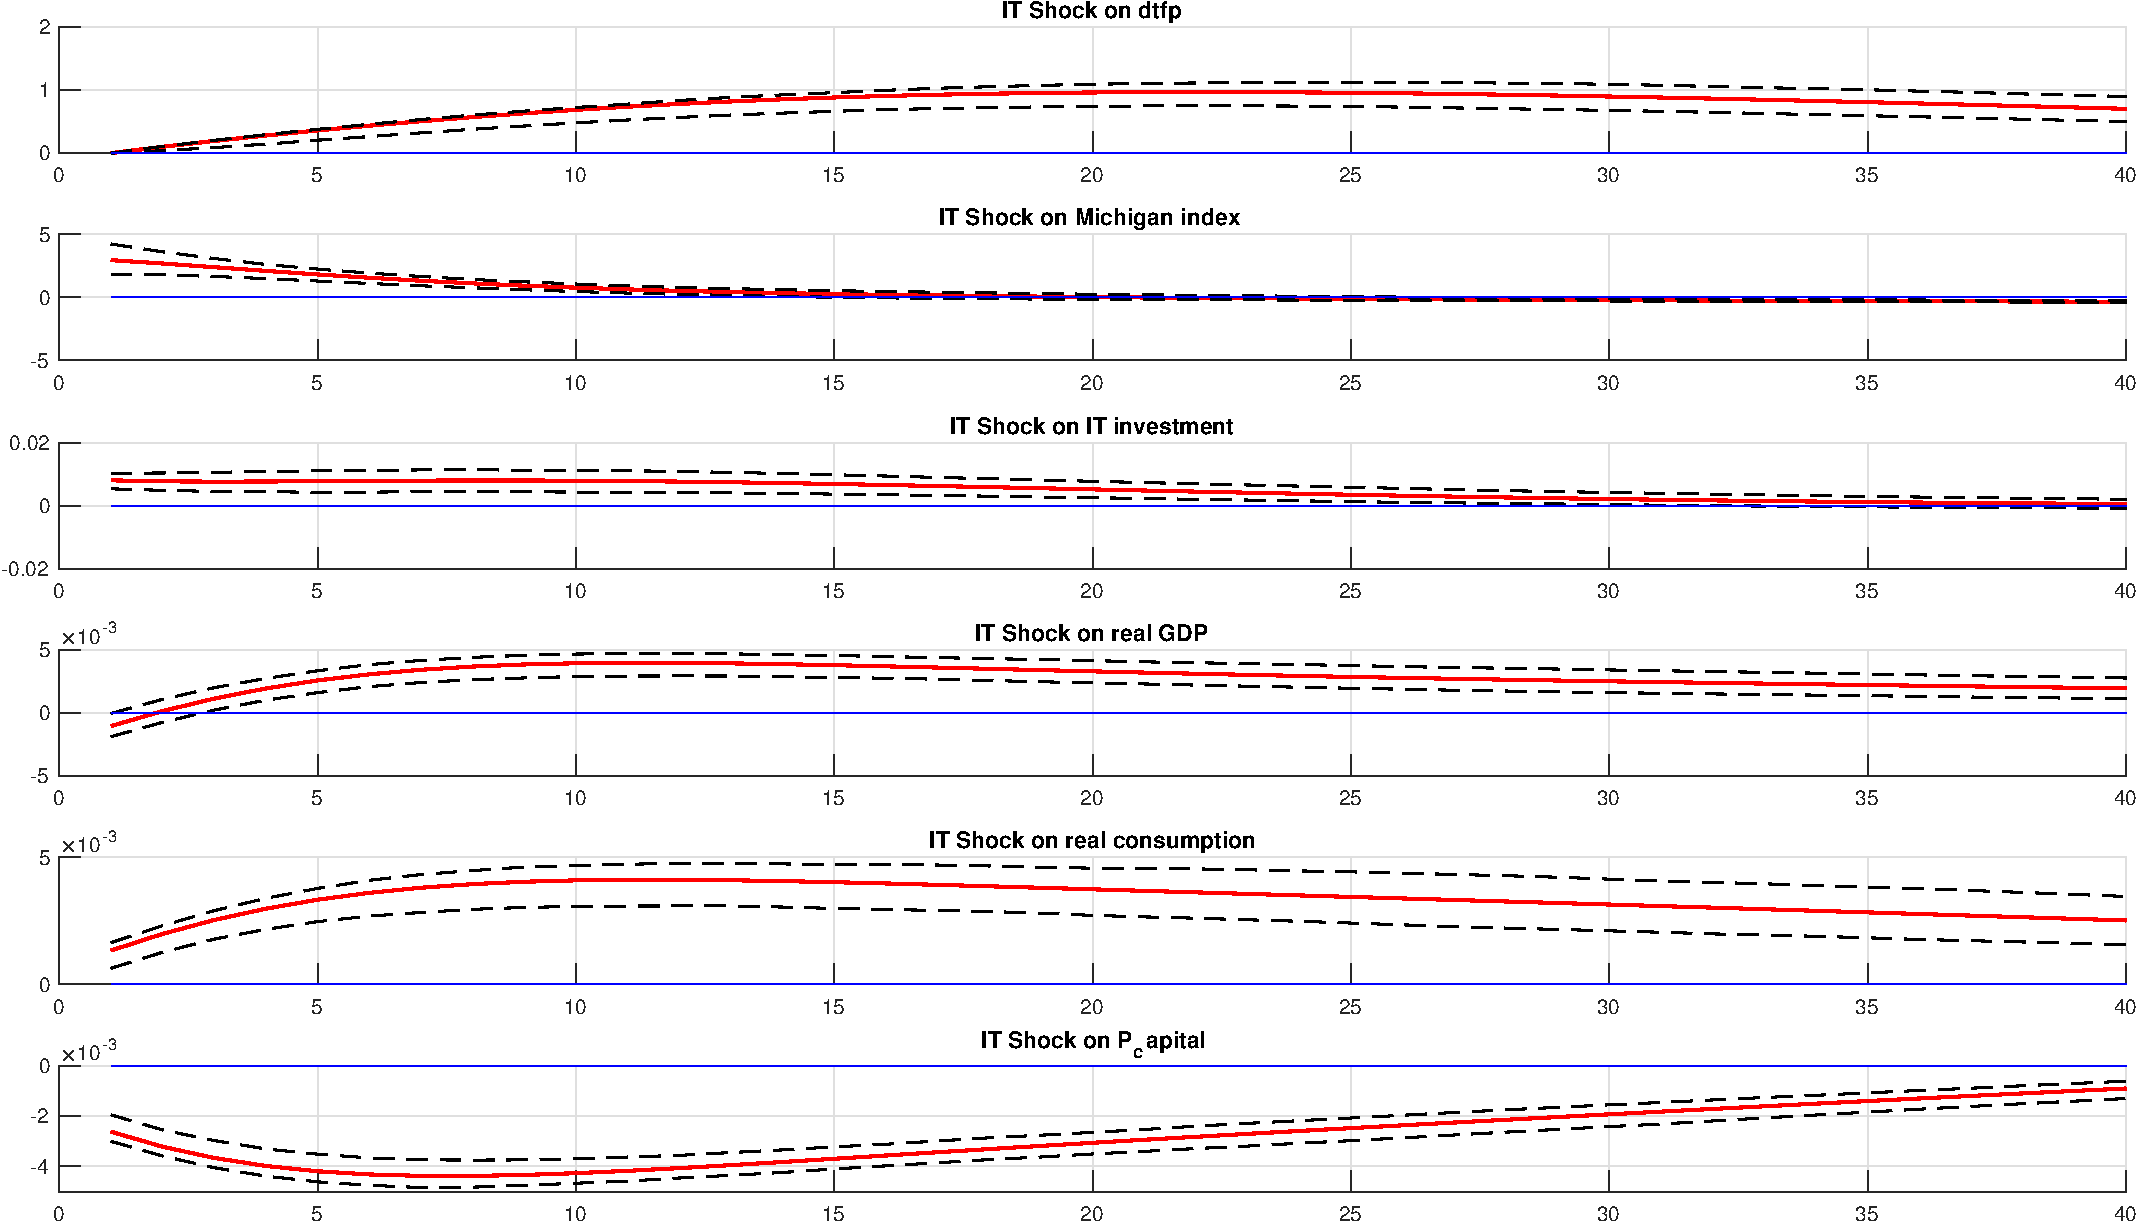
\includegraphics[width=8.5cm]{\ourFigPath Figures/fig_IT_Shock_Ryan_two_stepsID_24-Nov-2017_16_17_19}}
\end{figure}
	
	
		
	
	
\end{document}

